\chapter{A variant-dependent molecular clock with anomalous diffusion models SARS-CoV-2 evolution in humans}\label{ch:chapter2}

%% TODO:
% - Completar com más info donde esté marcado con "%%%"

\begin{flushright}
    \textit{Simplicity is prerequisite for reliability.}\\
    --- Edsger W. Dijkstra
\end{flushright}

\vspace{1cm}

\noindent This work has been published in a peer-reviewed journal. See the full citation:\\

\noindent \textbf{Goiriz L}, Ruiz R, Garibo-i-Orts O, Conejero J.A, Rodrigo G. (2023) \href{https://doi.org/10.1073/pnas.2303578120}{A variant-dependent molecular clock with anomalous diffusion models SARS-CoV-2 evolution in humans}. \textit{Proc. Natl. Acad. Sci. U.S.A.}, 120(30): e2303578120.\\

\noindent In this publication, I performed all the data analysis and figures, except for \textbf{Figure \ref{fig:fig2.2}} where OGO made contributions in the data analysis. The results were discussed with RR, JAC and GR. GR designed the research.

\vfill

\pagebreak

\sloppy

\section{Introduction}

Viruses lie at the frontier of living and inert matter, as they lack own metabolism to sustain replication but are subject to Darwinian evolution (\textit{i.e.}, mutation and selection) \cite{koonin2013}. As fast evolving biological agents \cite{drake1998}, they are ideal substrates from which to learn mechanisms that modulate genetic variation, as well as to test theoretical models of evolution. One important model is the molecular clock hypothesis, introduced by Emile Zuckerkandl and Linus
Pauling, which dates back to early times of molecular biology.

\begin{definition}[Molecular Clock Hypothesis (1965)]
    The molecular clock hypothesis states that the rate of evolution of a gene is constant over time. This implies that genes accumulate mutations at a constant rate, providing a molecular basis for measuring evolutionary timescales \cite{zuckerkandl1965,ayala1999,kumar2005}.
\end{definition}

Motoo Kimura further developed this theory into a comprehensive framework in known as the neutral theory of molecular evolution.

\begin{definition}[Neutral Theory of Molecular Evolution (1968)]
    The neutral theory of molecular evolution proposes that most evolutionary changes at the molecular level are caused by random genetic drift of selectively neutral mutants \cite{kimura1968,kimura1987}.
\end{definition}

Neutral theory of molecular evolution predicts, in addition, that such clocks are Poissonian stochastic processes (\textit{i.e.}, evolution seen as a Brownian motion with diffusivity such that mean and variance are equal) \cite{kimura1987}, a concept that will be elaborated upon in \textbf{Section \ref{sec:evolution-approximated-as-a-continuous-stochastic-process}}. Despite the results from seminal studies of some viral genes are in tune \cite{gojobori1990,leitner1999}, the molecular clock hypothesis still raises controversy \cite{kumar2005}, as evolution appears as a highly volatile and vagary stochastic process due to environmental changes, transmission bottlenecks, and recombination and speciation events. Indeed, such a null model can be rejected in numerous cases \cite{jenkins2002}, and overdispersed populations in genetic variation (\textit{i.e.}, with larger variance than mean) seem common across phyla \cite{bedford2008}. Nonetheless, without extensive monitoring of evolution in natural conditions for a reasonable period of time, it is difficult to describe the mathematical model underlying such stochastic dynamics.

The emergence (at the end of 2019) and global spread (during 2020) of severe acute respiratory syndrome coronavirus 2 (SARS-CoV-2) has caused the ongoing pandemic \cite{li2021}. Due to the high impact on public health, huge efforts have been carried out worldwide to sequence the whole viral genome from different patients in real time of pandemic \cite{bedford2020, lopez2021, lemieux2021, tegally2021, kraemer2021, rockett2022, jackson2021}. To date, more than 10 million sequences are available. Importantly, this has allowed tracking introductions and measuring the extent of virus transmission at the community level \cite{bedford2020}, assessing the effectiveness of containment strategies \cite{lopez2021}, realizing the impact of superspreading events \cite{lemieux2021}, identifying novel variants of concern and their key mutations \cite{tegally2021}, monitoring spatiotemporal invasion dynamics of specific variants \cite{kraemer2021}, disclosing co-infection occurrences with different variants \cite{rockett2022}, and discovering the circulation of recombinant viruses, which might lead to increased infectiousness or pathogenicity \cite{jackson2021}. In addition, computational analyses have shown that SARS-CoV-2 primary evolves under purifying selection in humans, with some sites displaying adaptation \cite{rochman2021}. They have also shown that the spectrum of acquired mutations is greatly asymmetric (\textit{viz.}, dominated by C$>$U and G$>$U substitutions) \cite{yi2021}. Notwithstanding, a detailed study of the stochastic dynamics underlying such evolutionary motion to assess fundamental scaling laws and conditions for criticality has not been carried out.

In this work, we exploited the unprecedented monitoring of the evolution of a human virus in nature to conduct a study aimed at describing this process as a (non-)Brownian motion, considering the number of acquired mutations as the displacement of the viral particle from the origin (\textbf{Fig. \ref{fig:fig2.1}}). For that, several biostatistical analyses over millions of whole genome sequences at the ensemble level were evaluated on the basis of a time-dependent probabilistic mathematical model, without relying on phylogeny. Of note, our results challenge the conventional molecular clock hypothesis by providing new theoretical foundations for viral evolution. 

\begin{figure}[ht!]
    \centering
    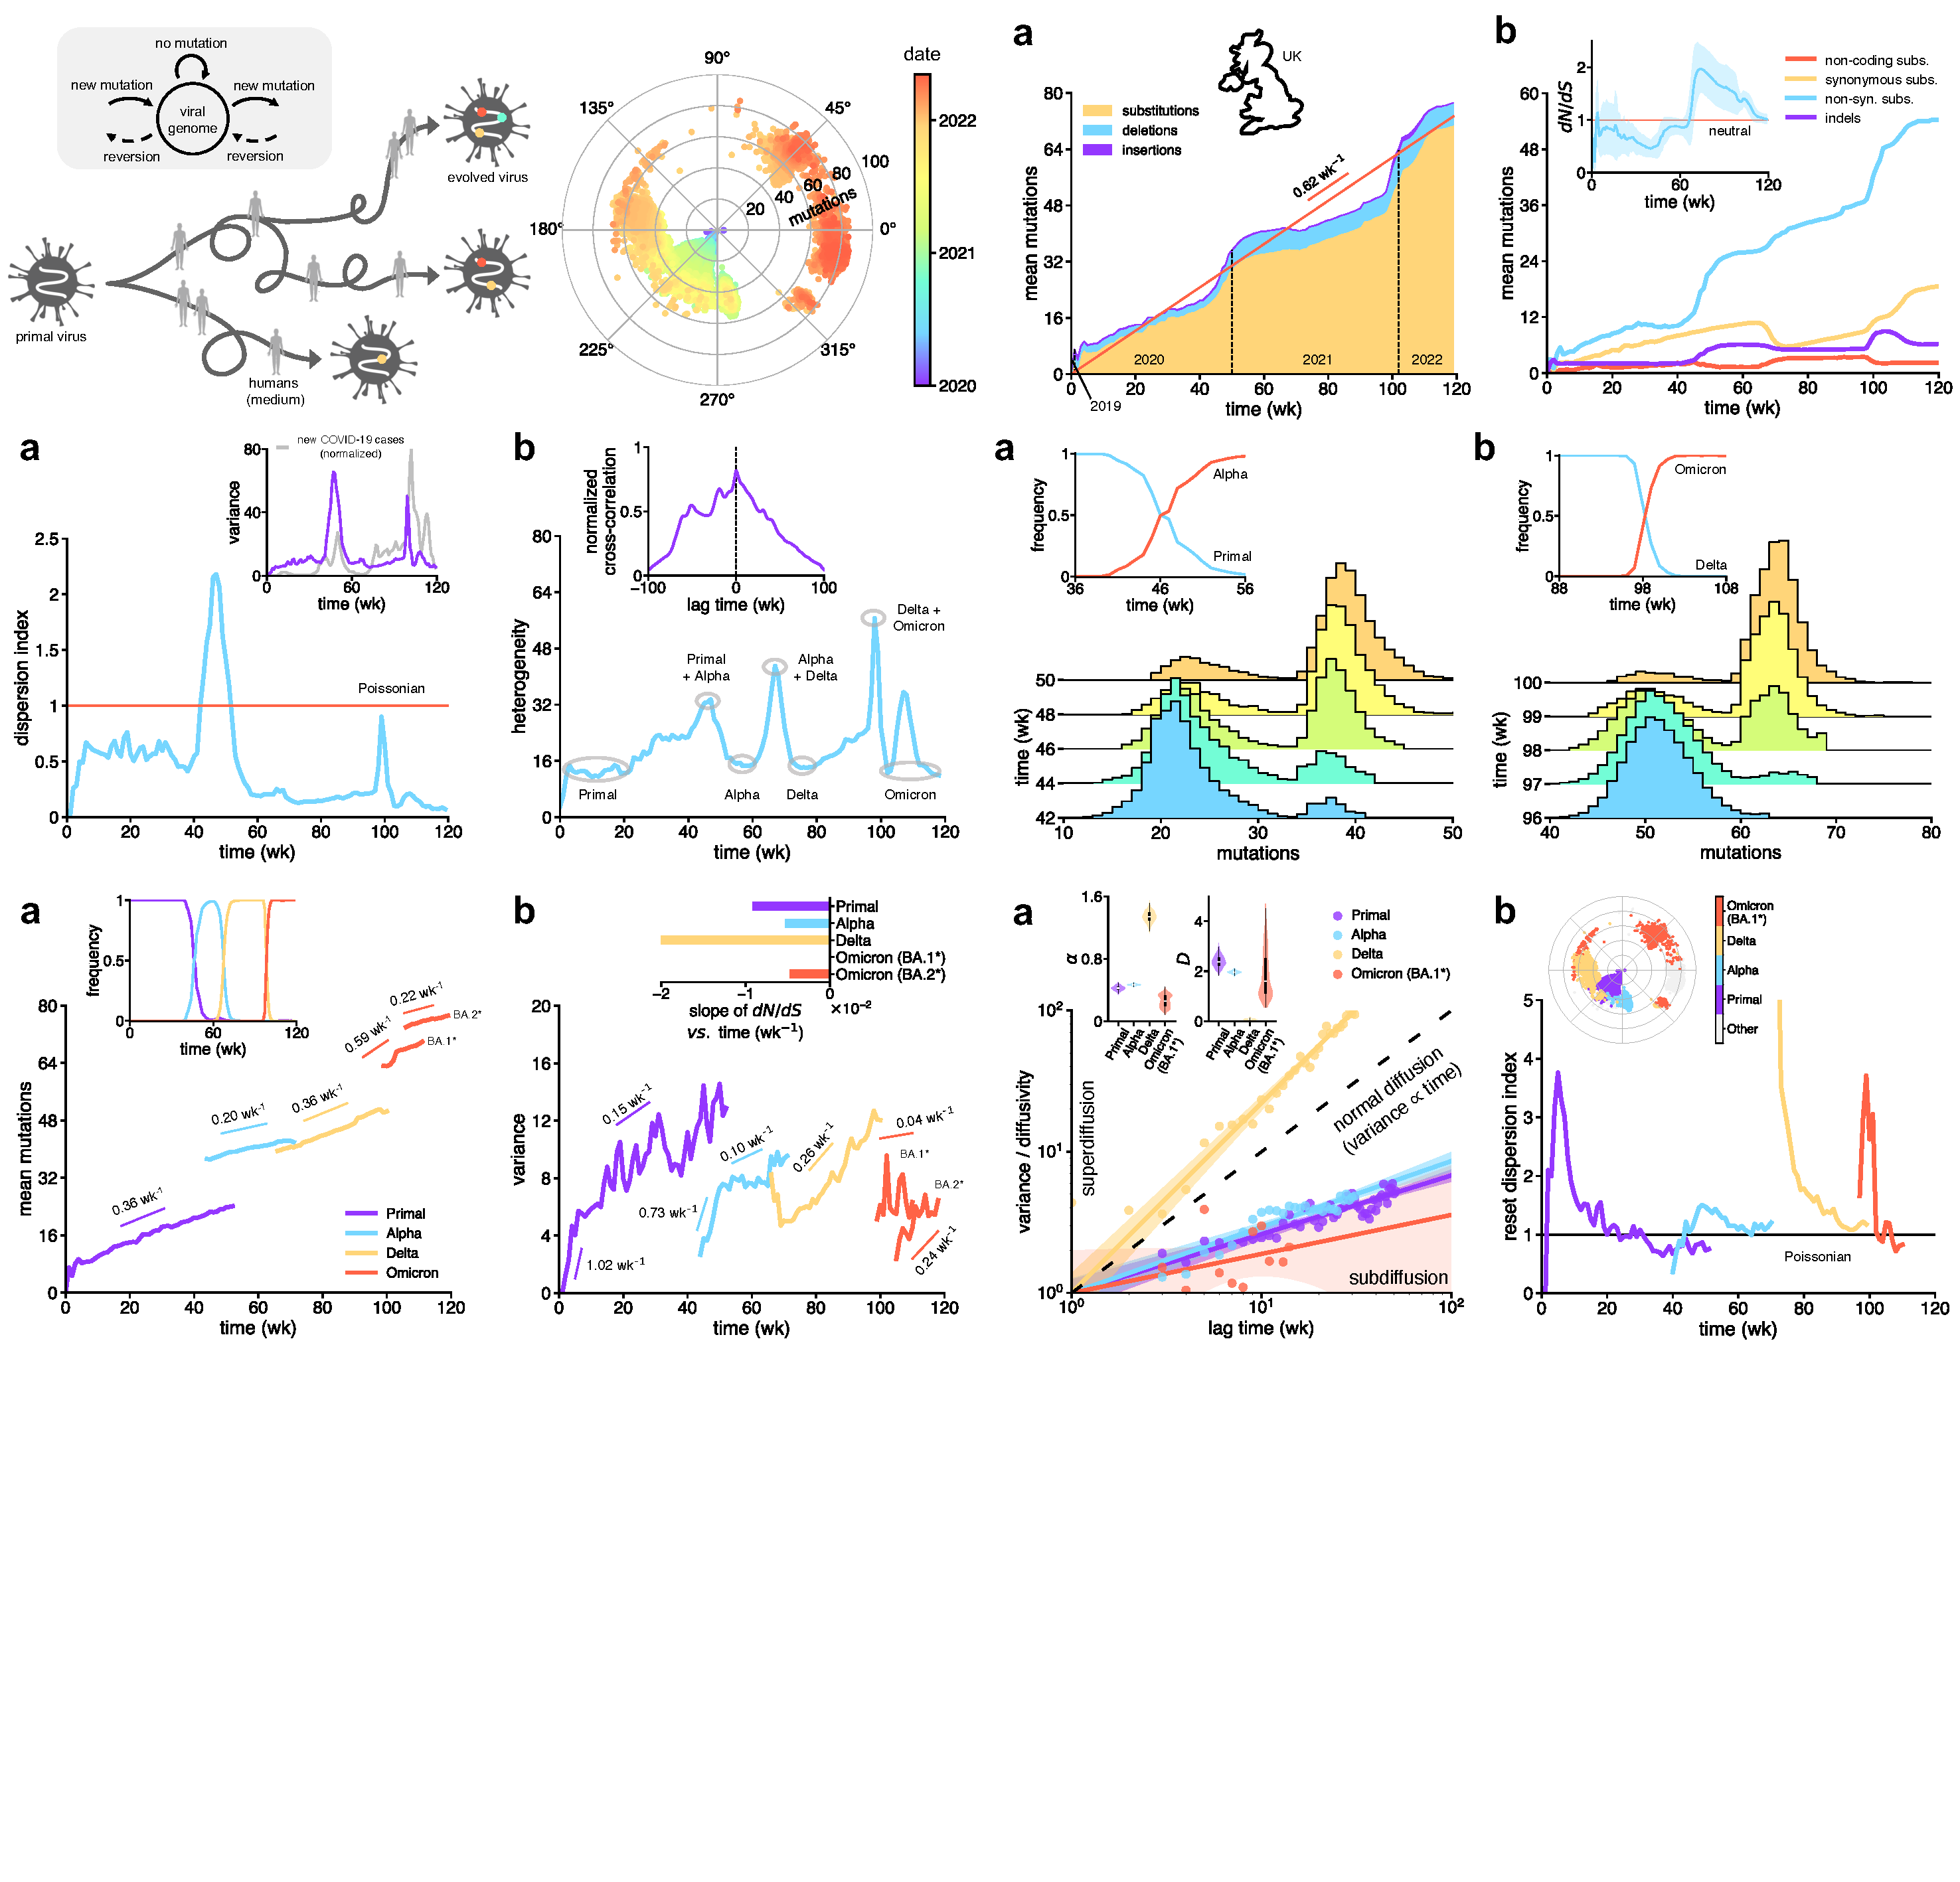
\includegraphics[trim={0 37.5cm 36.5cm 0.5cm},clip, width=0.67\linewidth]{assets/Ch2Fig.pdf}
    \caption{Schematics of the evolutionary motion of the virus (viewed as a stochastic process). Inset: associated state-transition diagram.}\label{fig:fig2.1}
\end{figure}
\vfill
\section{Results}\label{sec:results}

We sought to characterize the mean and variance (mean squared displacement) of the overall stochastic process by which the observable viral genome accumulates mutations with time (since the emergence in Wuhan, China). This was modeled in a continuous form by the Langevin equation:

\begin{equation}
    \frac{dm(t)}{dt}=\kappa + \xi(t)\label{eq:solution-model},
\end{equation}

\noindent where $m(t)$ is the total number of mutations in the genome at time $t$, $\kappa$ the evolution rate (which could be time-dependent), and $\xi(t)$ an integrative noise source whose properties shape the evolutionary motion.

Due to the large number of available SARS-CoV-2 sequences from United Kingdom (UK), our analysis was focused on this country. Using landmark multidimensional scaling (LMDS) \cite{deSilva2003}, we obtained a representation of all available genotypes in a two-dimensional space (\textbf{Fig. \ref{fig:fig2.2}}), which served to appreciate the virus evolution as a complex diffusion process. In this polar plot, the radius represented the number of mutations and the angle encompassed the rest of sequence variation.

\begin{figure}[ht!]
    \centering
    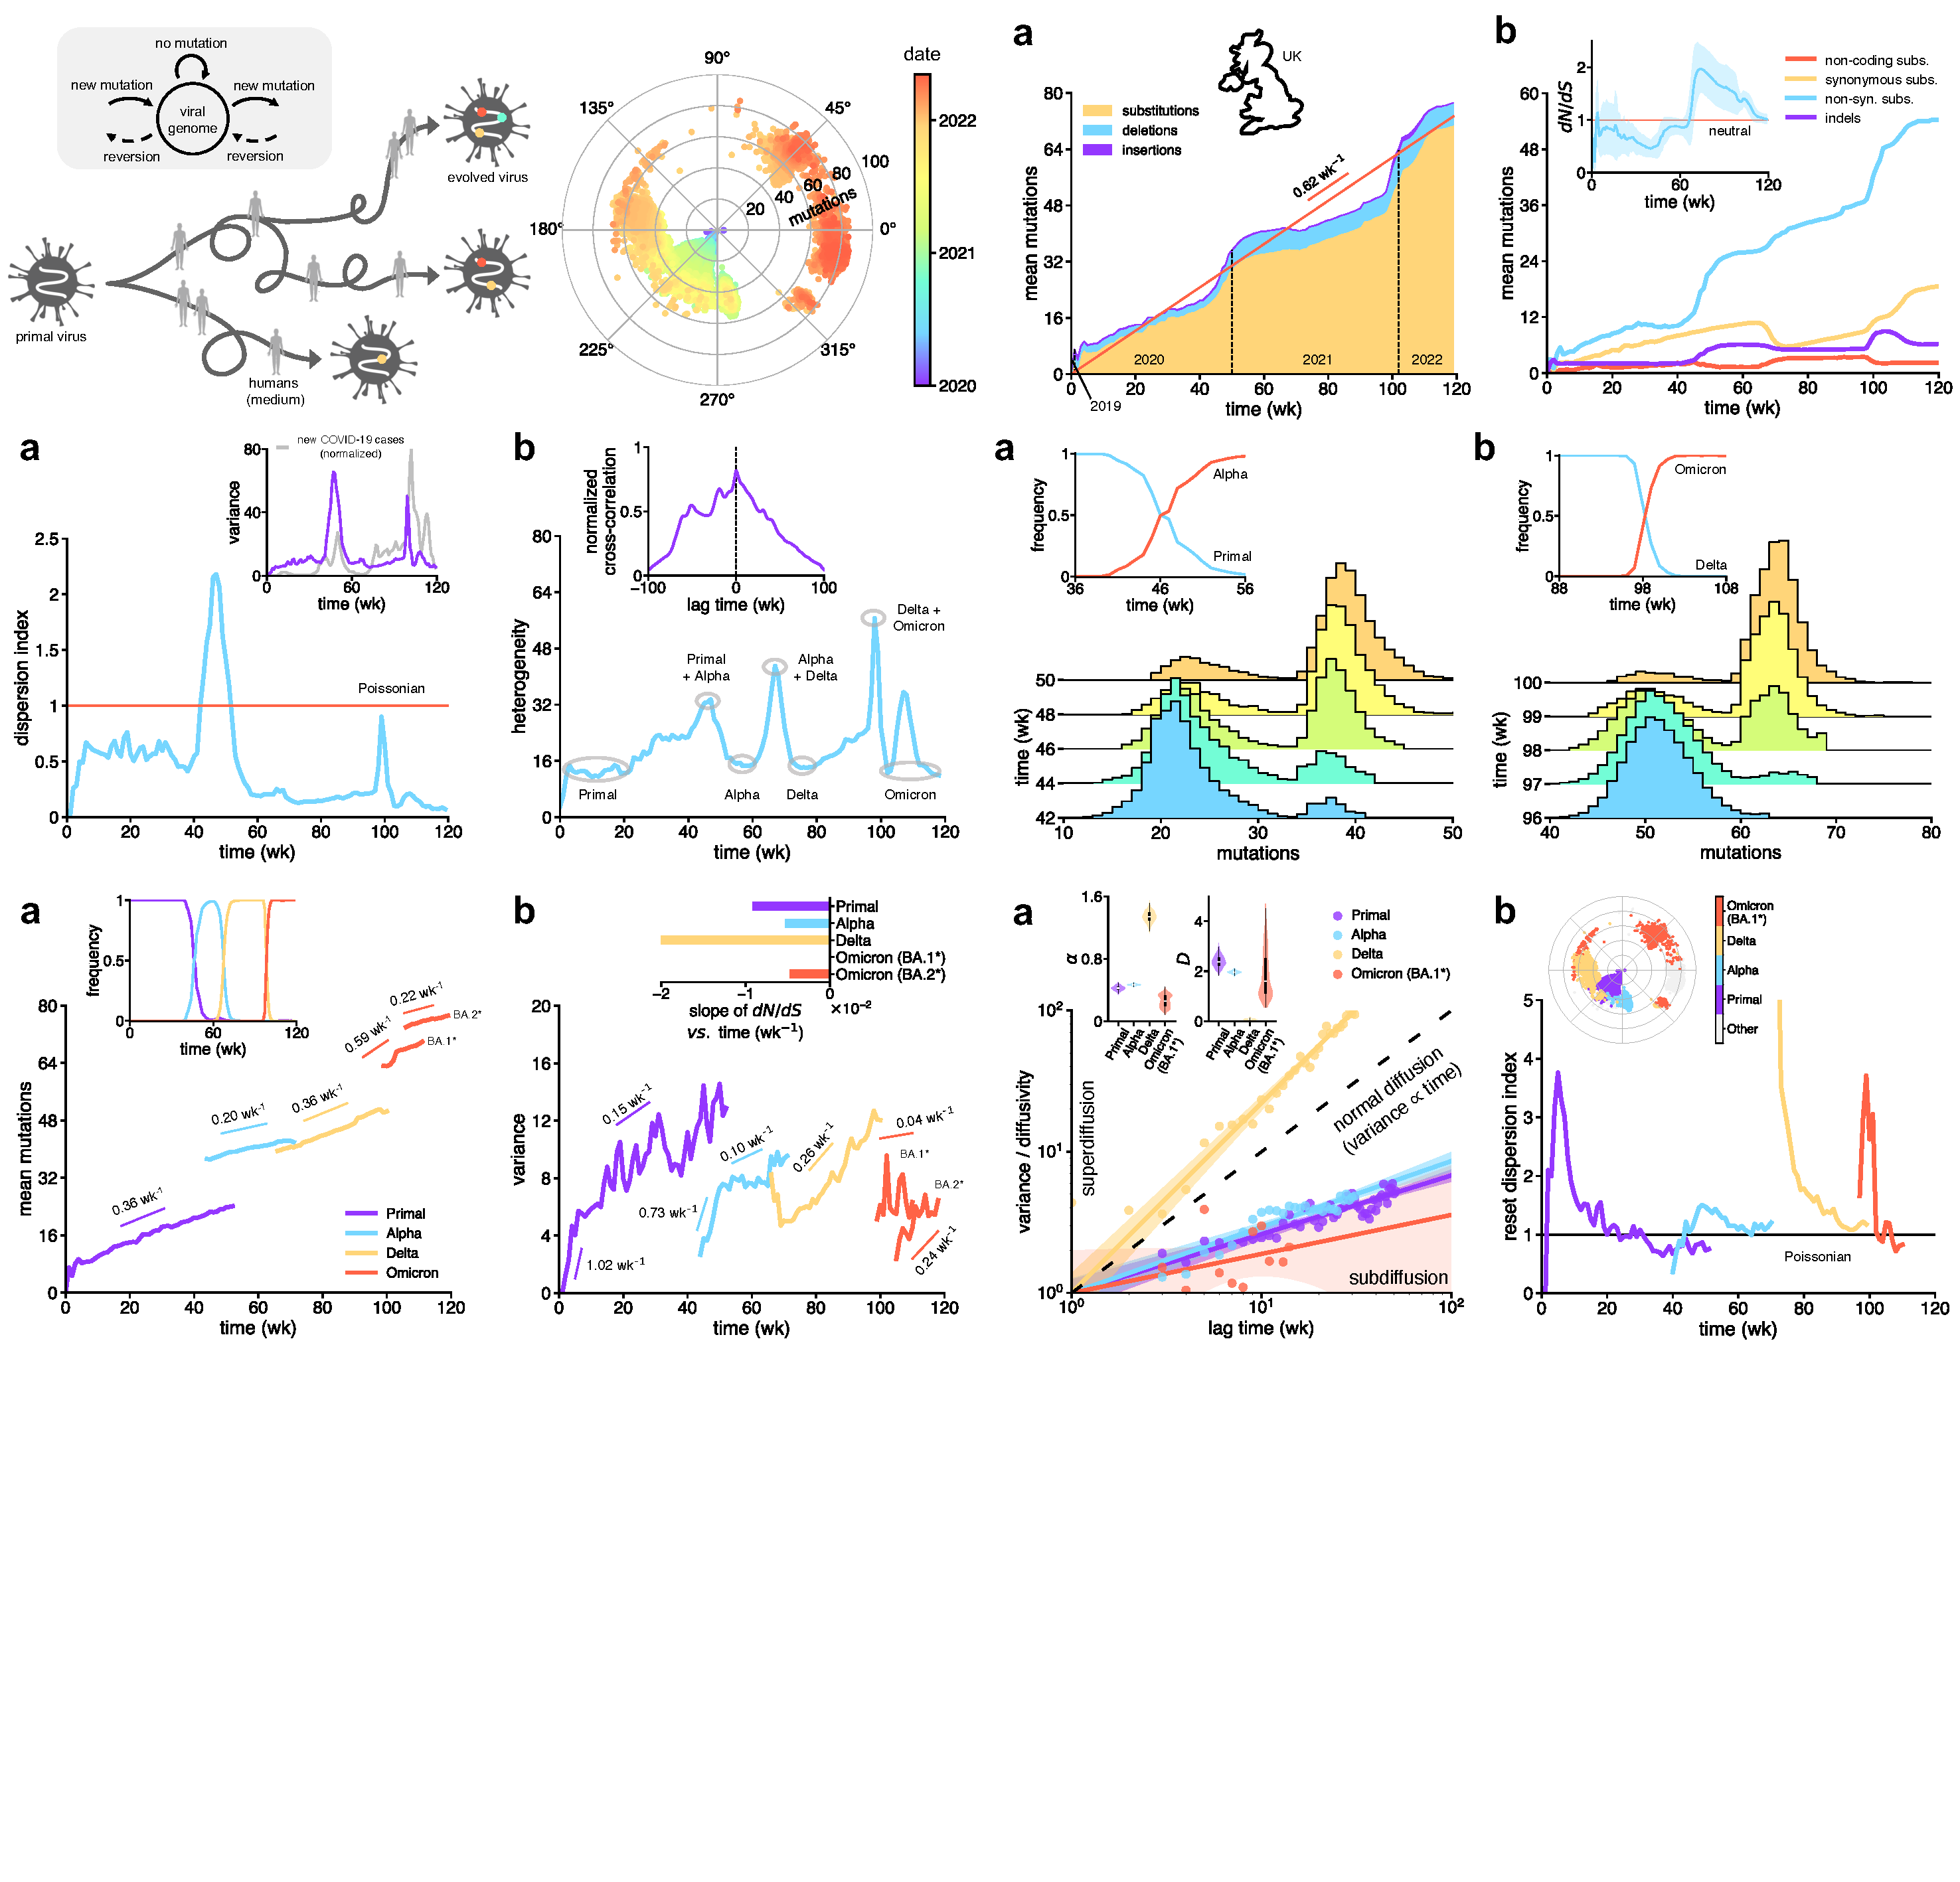
\includegraphics[trim={13.533cm 37.5cm 25.1cm 1cm},clip, width=0.5\linewidth]{assets/Ch2Fig.pdf}
    \caption{2D projection of all viral sequences colored by date.}\label{fig:fig2.2}
\end{figure}

To characterize the stochastic process, we first quantified the rate at which the viral genome accumulates a mean number of mutations with time. Considering all types of mutations and discretizing time by weeks (\textit{i.e.}, all sequences available in a week were pooled together), we obtained a macroscopic evolution rate of 0.62 wk\textsuperscript{-1} (Pearson's correlation with no intercept, $P < 10^{-4}$; \textbf{Fig. \ref{fig:fig2.3}a}). Substitutions were much more frequent than insertions and deletions (indels). However, at some points (at the end of 2020 and of 2021), an acceleration in the evolution rate was observed, thereby deviating from a molecular clock model with constant rate. Yet, without phylogenetic inference, this picture just reflected population changes and not strict evolutionary paths. In addition, mutations were classified according to their type (\textit{viz.}, non-coding, synonymous, non-synonymous, and indels), and the ratio between the number of nonsynonymous and synonymous substitutions per site (dN/dS) was estimated (\textbf{Fig. \ref{fig:fig2.3}b}), which is a common tool to assess the strength and mode of natural selection \cite{nielsen2005}. The observed dN/dS signature (fluctuation around 1 over time) suggested evolution under purifying selection of a series of adapted variants.

\begin{figure}[ht!]
    \centering
    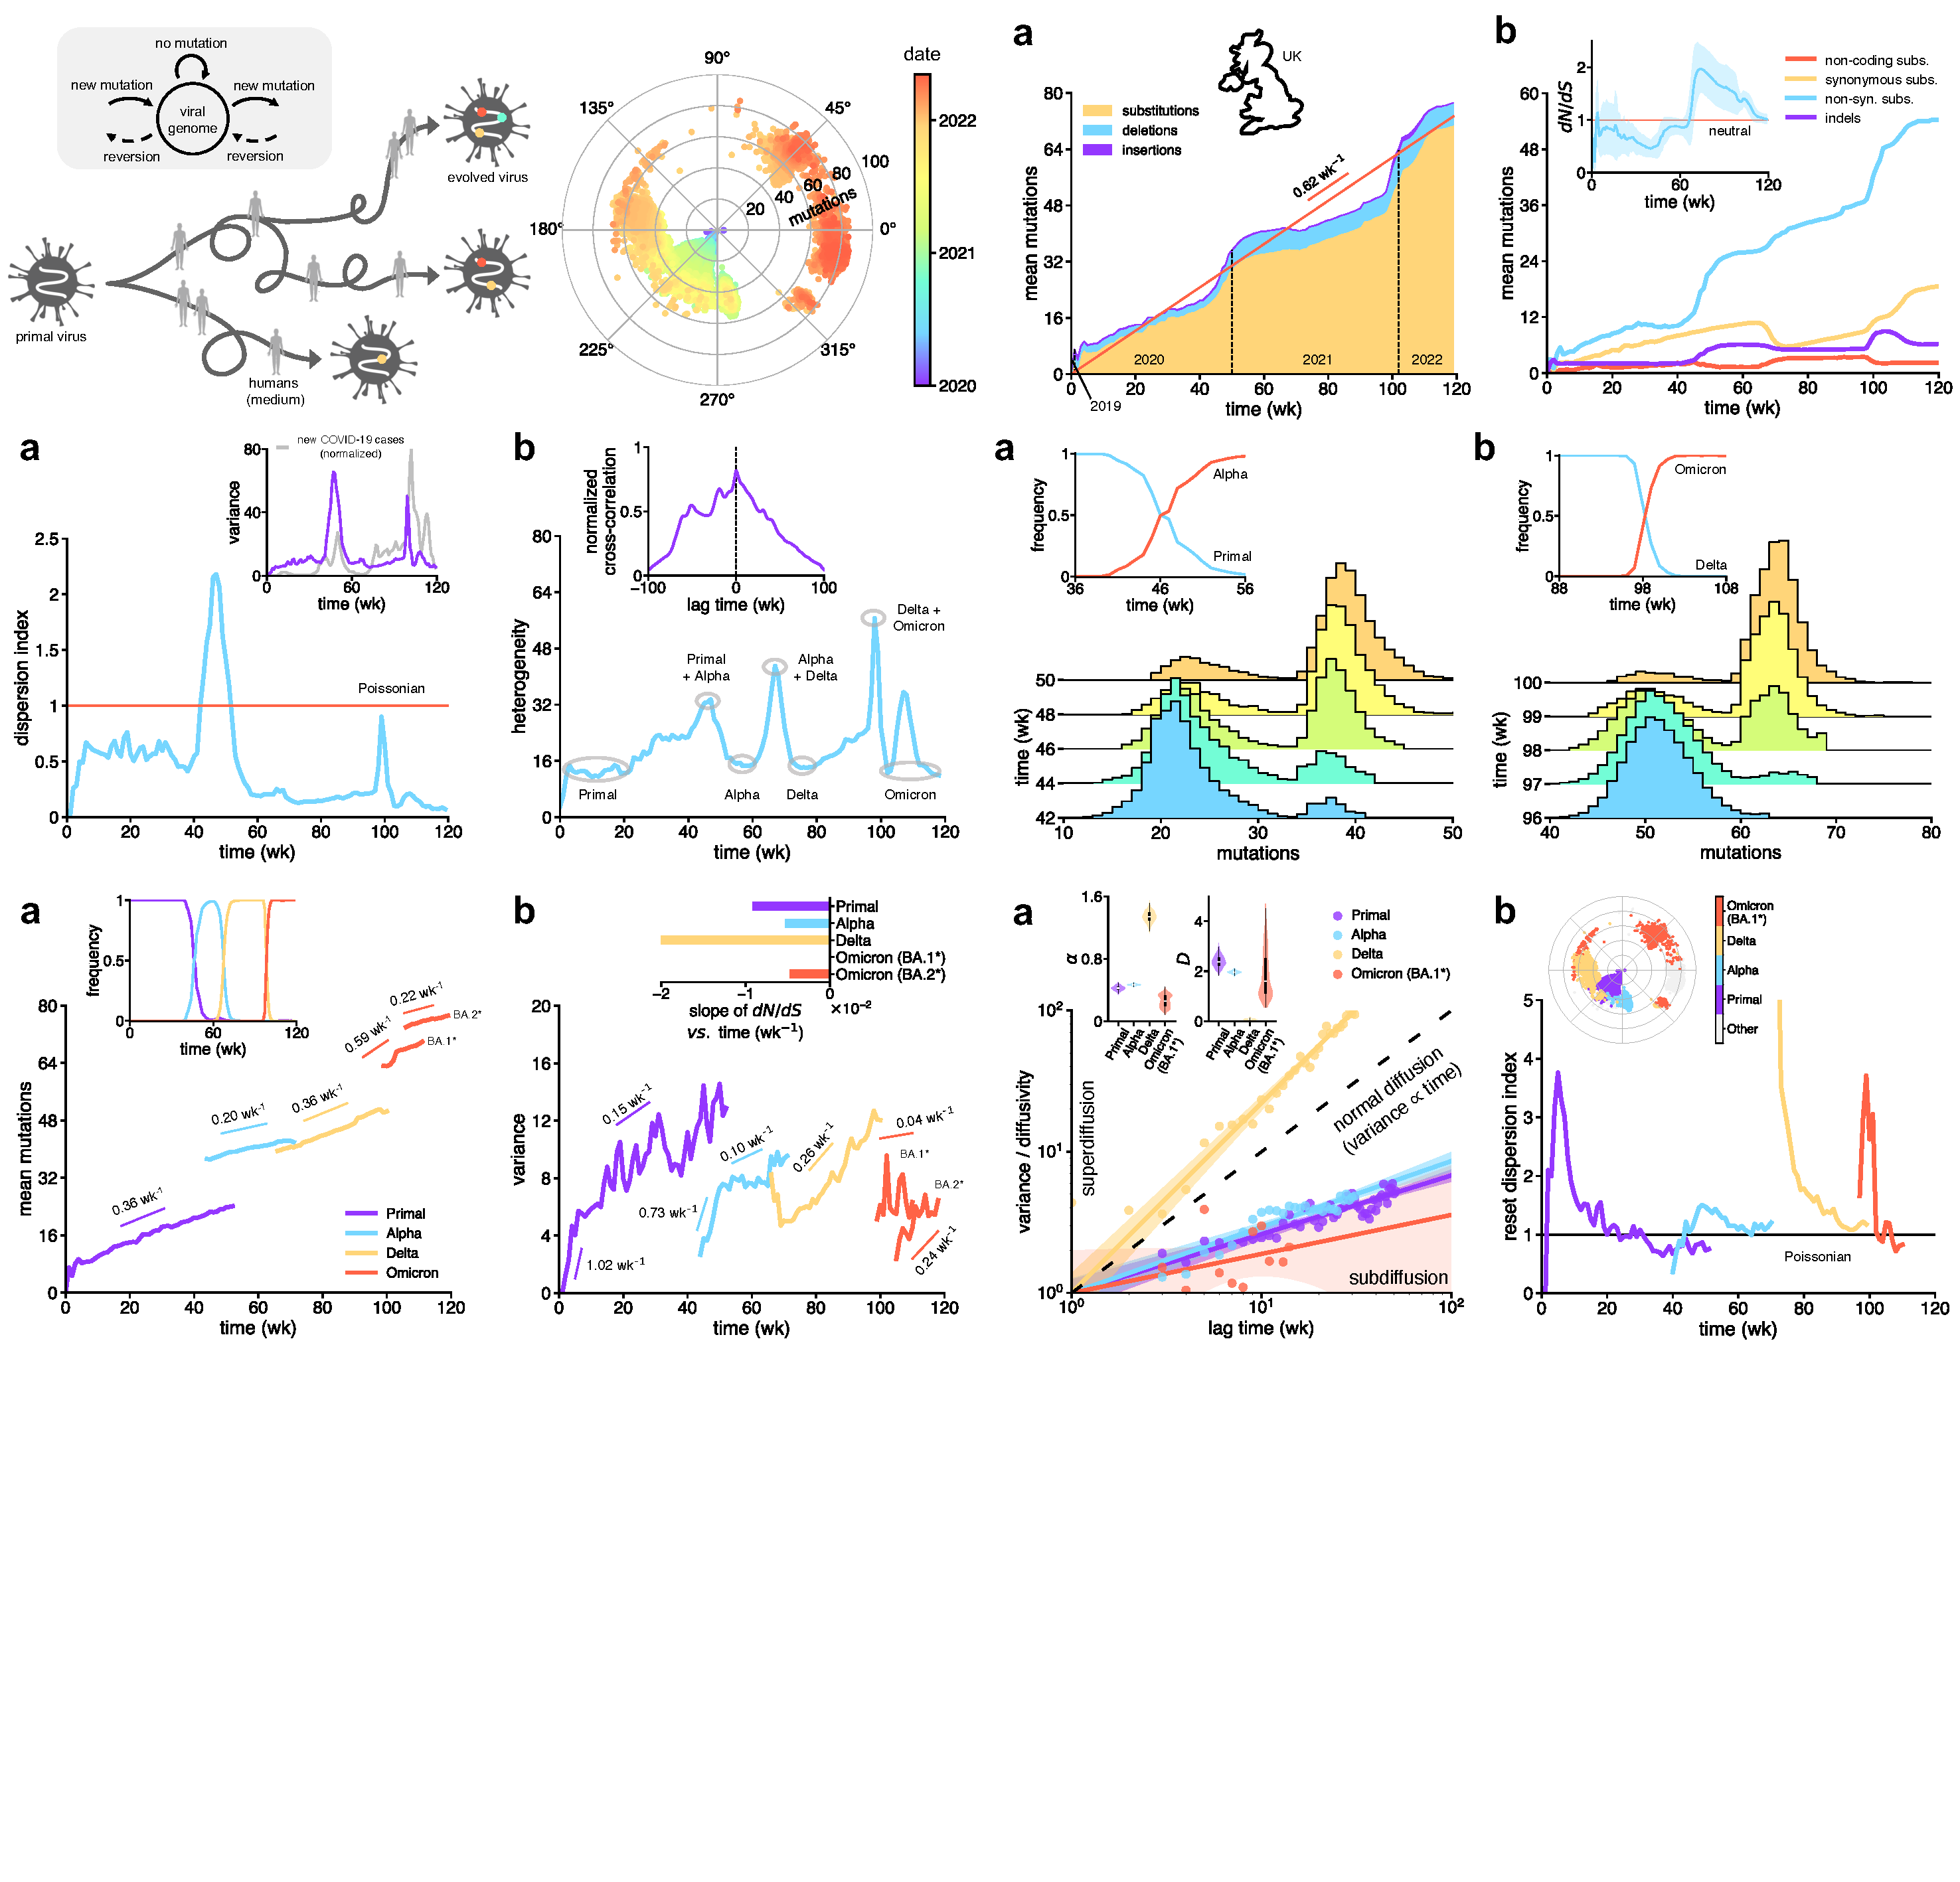
\includegraphics[trim={25.8cm 37cm 0 0.2cm},clip, width=\linewidth]{assets/Ch2Fig.pdf}
    \caption{a) Time-course of the mean number of accumulated mutations in the viral genome, distinguishing between substitutions, deletions, and insertions. Linear regression over the total shown in red (R\textsuperscript{2} = 0.95). b) Time-course of the mean number of non-coding substitutions, synonymous substitutions, non-synonymous substitutions, and indels. Inset: dN/dS with time (mean plus/minus standard deviation).}\label{fig:fig2.3}
\end{figure}

To test whether the accumulation of mutations in SARS-CoV-2 was a Poissonian stochastic process, we also calculated the variance and the dispersion index, understood as the ratio between variance and mean (\textbf{Fig. \ref{fig:fig2.4}a}). The study of the variance is often overlooked, despite it is essential to comprehend the evolutionary motion. We found largely sub-Poissonian dynamics (\textit{i.e}., dispersion index $<$ 1) with two main dispersion bursts at the times at which the evolution rate was accelerated. To inspect the origin of such a dynamic profile, we performed a sequence classification into variants. For simplicity, four variants were considered, \textit{viz.}, Primal, Alpha, Delta, and Omicron.

We realized that the first dispersion burst corresponded to the transition from Primal to Alpha, while the second to the transition from Delta to Omicron (\textbf{Fig. \ref{fig:fig2.4}b}). The number of new coronavirus disease 2019 (COVID-19) cases also correlated with the variance (inset of \textbf{Fig. \ref{fig:fig2.4}a}). Representing the distributions of accumulated mutations with time, we disclosed a bimodal behavior during such transitions (\textbf{Fig. \ref{fig:fig2.5}a, b}), explaining the increased dispersion. The invading genotypes carried about 15-20 more mutations on average. Moreover, the transition from Alpha to Delta only generated a slight dispersion signal because both variants carried a similar number of mutations. Arguably, outlier SARS-CoV-2 genotypes in the existing distribution at a time led to the emergence of new variants, and the observed accelerations in evolution rate came from the inherent stochasticity of the evolutionary motion followed by rapid, mostly deterministic invasion events once a particular genotype acquired a selective advantage, such as higher transmissibility \cite{kraemer2021}. 

\begin{figure}[t]
    \centering
    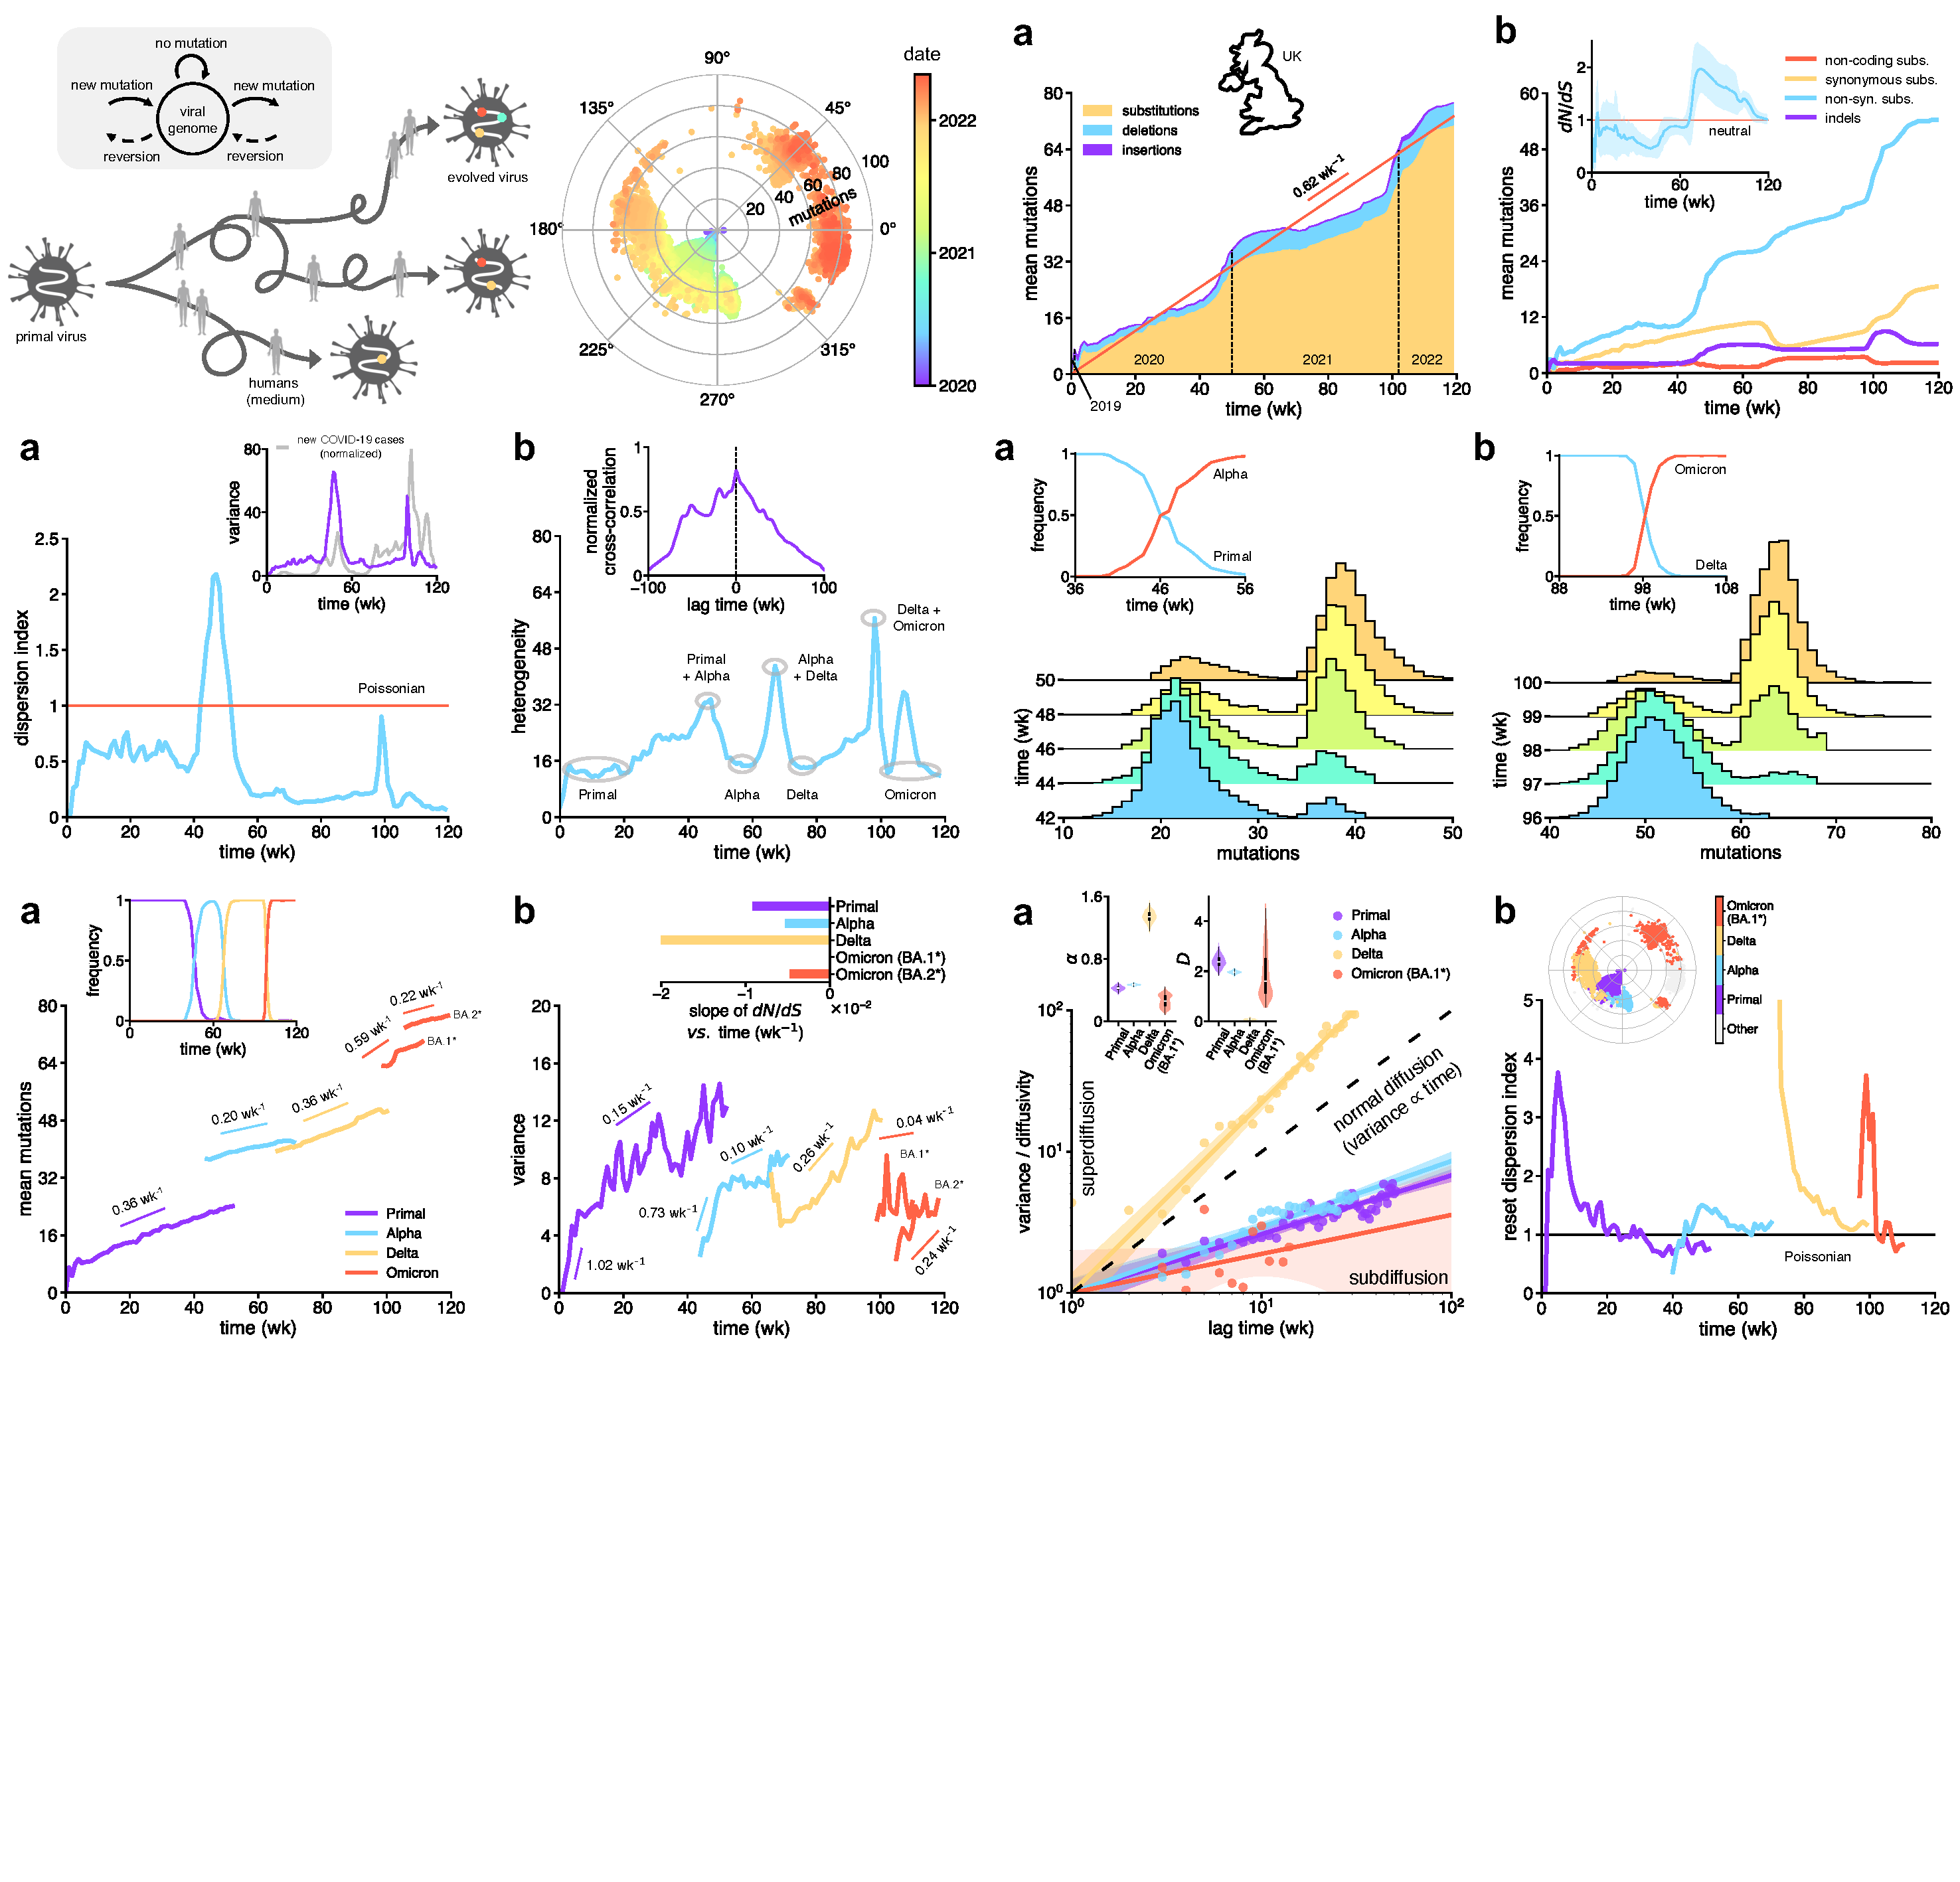
\includegraphics[trim={0.2cm 26cm 25.35cm 11cm},clip, width=\linewidth]{assets/Ch2Fig.pdf}
    \caption{a) Time-course of the dispersion index (variance/mean). Inset: variance with time; the normalized number of new COVID-19 cases is superimposed. b) Time-course of the degree of heterogeneity (mean Hamming distance), showing the different stages of the virus population in terms of variants. Inset: normalized cross-correlation between variance and heterogeneity with time.}\label{fig:fig2.4}
\end{figure}

Due to the virus population reset caused by the invasion of a new variant, we calculated the time-dependent statistics per variant. The analyses conducted for each variant were independent from each other by considering subsets of properly annotated sequences (\textit{i.e.}, no evolutionary paths between variants were considered). Of note, the evolution rates of Primal, Alpha, and Delta were substantially lower (up to 0.36 wk\textsuperscript{-1} ) than the inferred macroscopic value of 0.62 wk\textsuperscript{-1} (\textbf{Fig. \ref{fig:fig2.6}a}), in agreement with previous estimates following phylogenetic methods \cite{ghafari2022}. In the dataset, Omicron was composed of two lineages with sufficient dissimilarity, \textit{viz.}, BA.1 and BA.2 (BA.1 displaced Delta and BA.2 displaced BA.1). Performing a decomposition, we observed that BA.1 evolved faster than BA.2 in UK.\\

\begin{figure}[ht!]
    \centering
    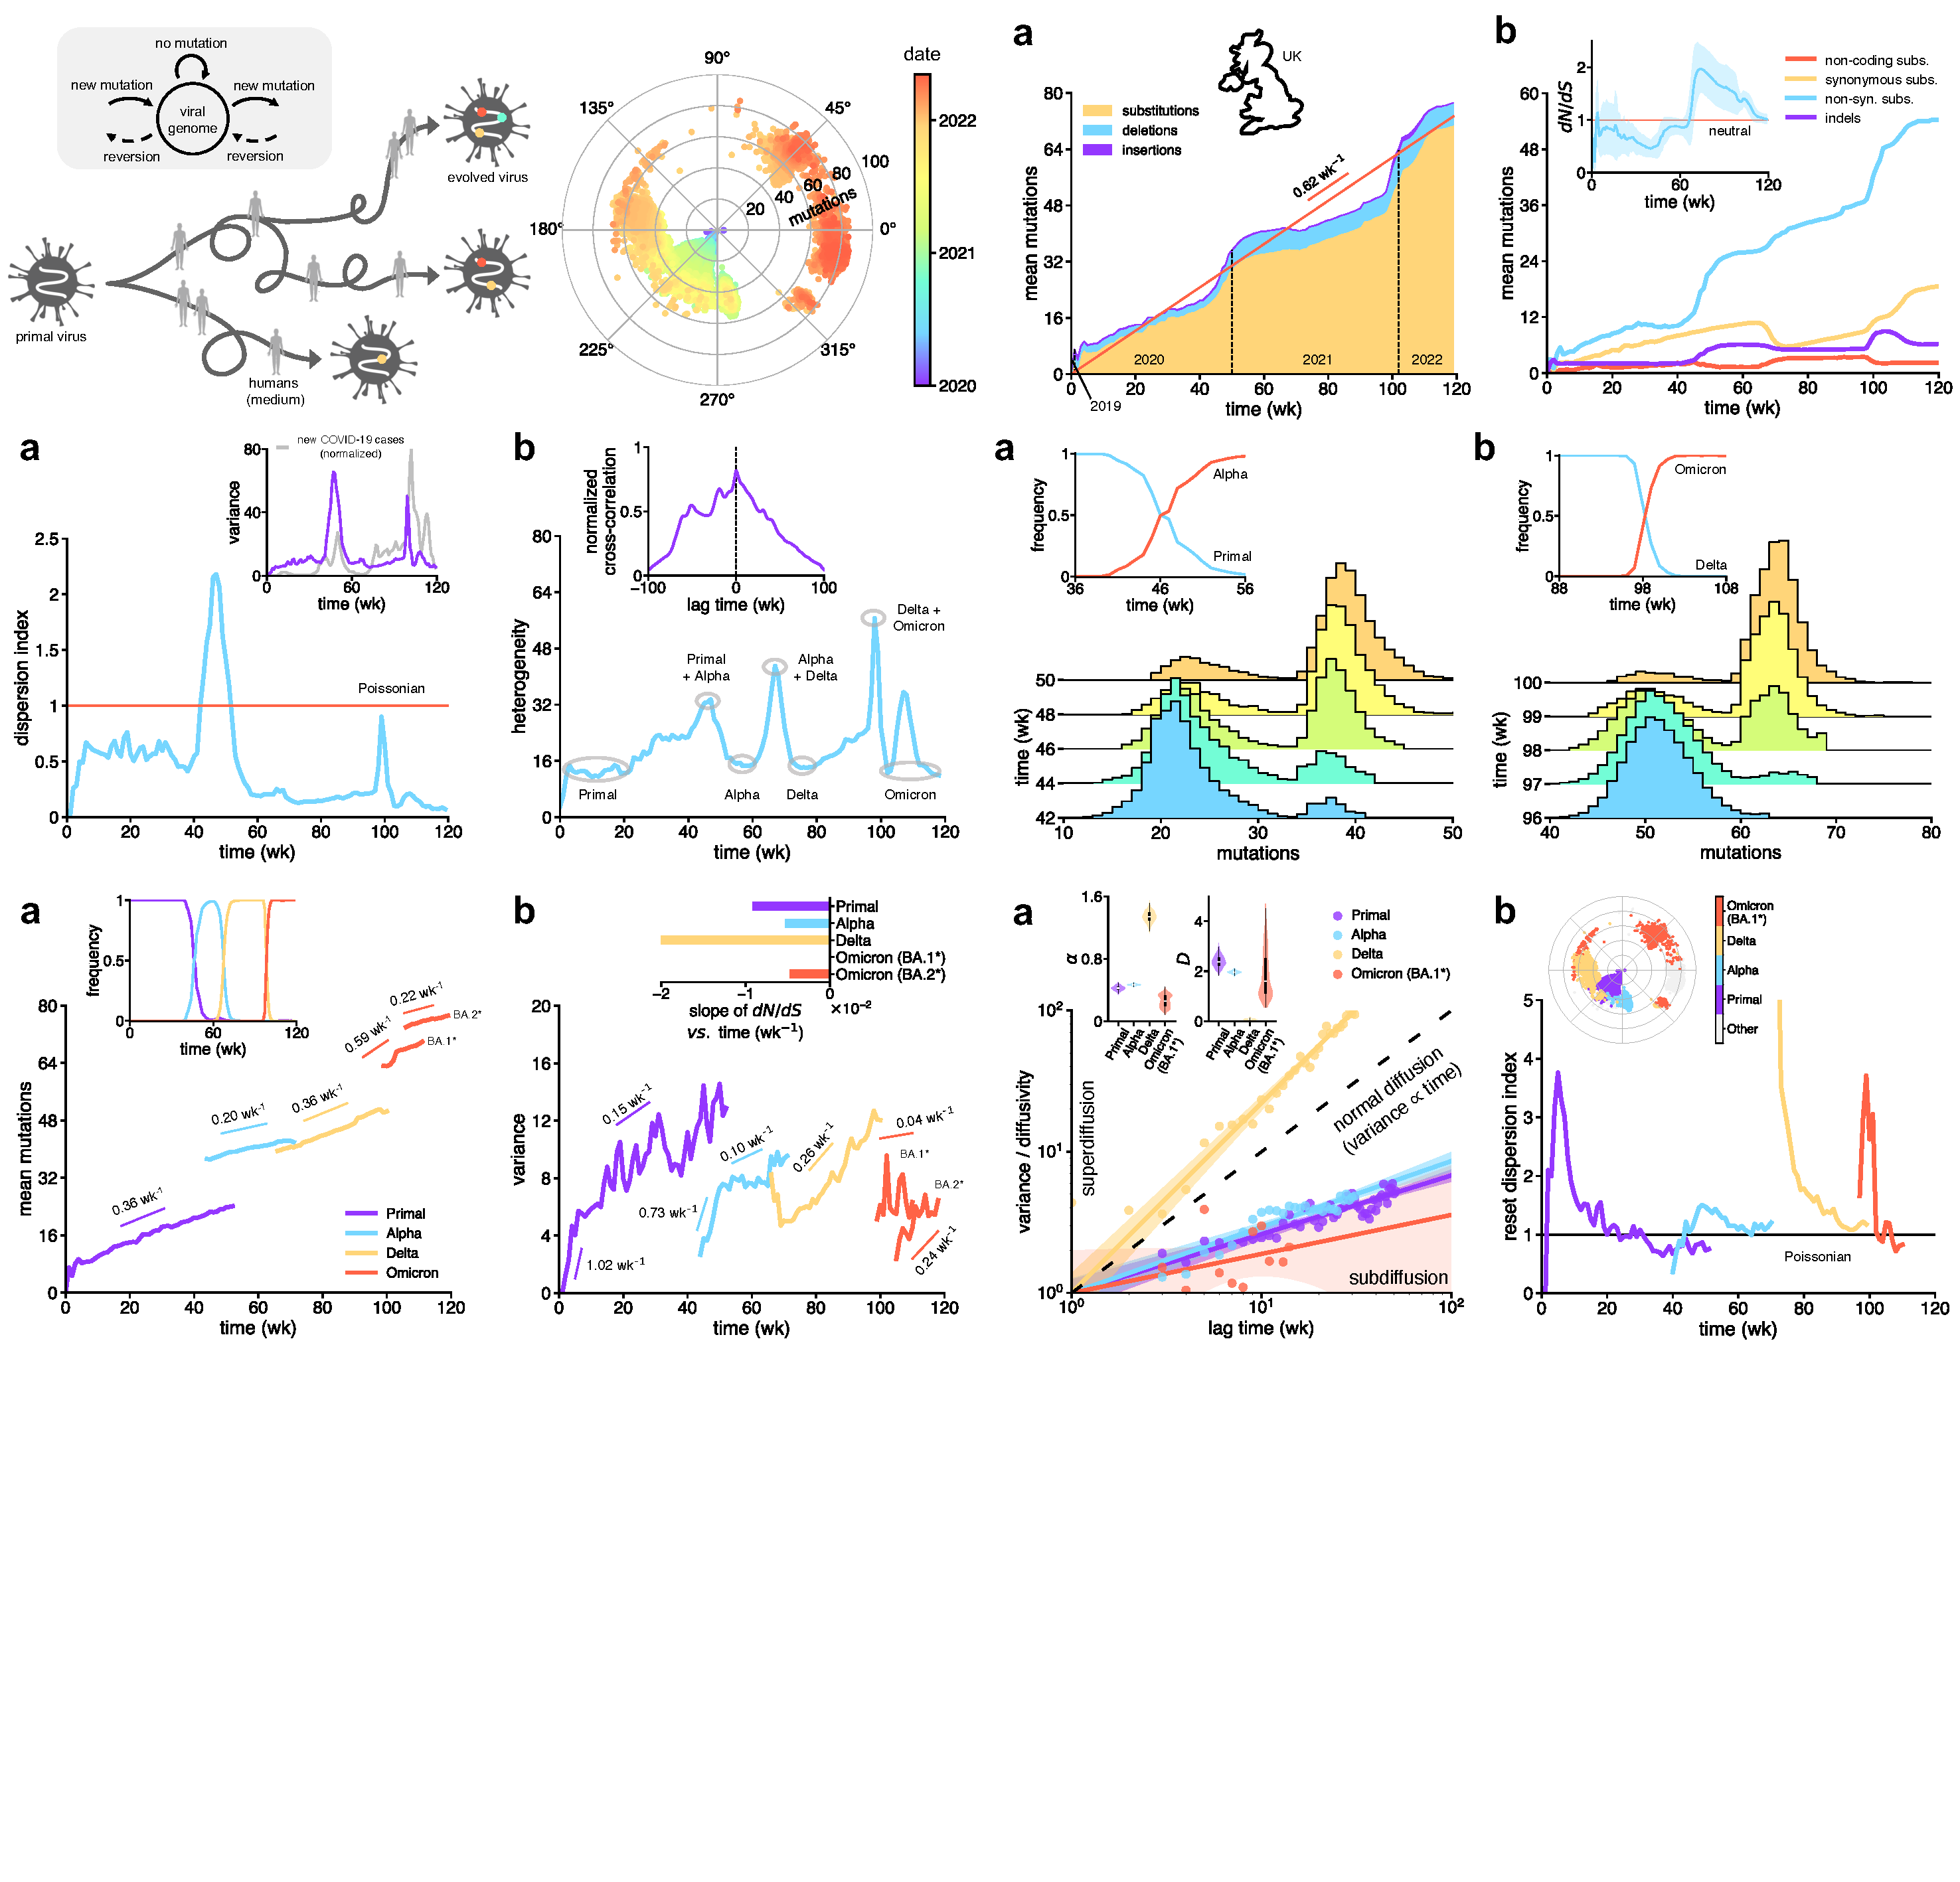
\includegraphics[trim={25.3cm 26cm 0.3cm 11cm},clip, width=\linewidth]{assets/Ch2Fig.pdf}
    \caption{Probability-based histograms of the number of accumulated mutations during the transition from Primal to Alpha (a) and Delta to Omicron (b). Insets: population frequency of the variants with time.}\label{fig:fig2.5}
\end{figure}

Collectively, the mean evolutionary motion was well captured by

\begin{equation}
    \mathbb{E}\left[m(t)\right] = \kappa t,
\end{equation}

\noindent with a constant variant-dependent rate, considering $\mathbb{E}\left[\xi (t)\right] = 0$ (Pearson's correlations, $P < 10^{-4}$ in all cases). In addition, we found significant nonlinear dependencies of the variance with time in all cases (Fisher-Snedecor's $F$ tests, $P < 10^{-4}$ for Primal, Alpha, and Delta, $P = 0.027$ for Omicron BA.1, and $P = 0.0003$ for Omicron BA.2; \textbf{Fig. \ref{fig:fig2.6}b}), which indicated a stochastic behavior with anomalous diffusion \cite{manzo2015}. In other words, SARS-CoV-2 underwent a non-Brownian evolutionary motion. This exciting result entailed that the explorations of the genotypic space by the virus to discover new phenotypes at different times were not fully uncorrelated within a clade.

To provide a quantitative picture of the process, we fitted $\mathbb{V}\left[m(t)\right]$ to the general expression $Dt^\alpha$, where $D$ is the diffusion coefficient and $\alpha$ the diffusion exponent. This expression is derived using the approaches shown in \textbf{Section \ref{sec:evolution-approximated-as-a-continuous-stochastic-process}} by considering 

\begin{equation}
    \text{Cov}\left[\xi(t),\xi(s)\right] = \frac{1}{2}D\alpha (\alpha - 1)\left|t - s\right|^{\alpha - 2}
\end{equation}

\noindent as the covariance function of the noise source $\xi(t)$. We found subdiffusion ($\alpha$ = 0.42, $\alpha$ = 0.47, and $\alpha$ = 0.28, respectively) in the cases of Primal, Alpha, and Omicron BA.1, while weak superdiffusion ($\alpha$ = 1.34) in the case of Delta (Pearson's correlations in log scale, $P < 10^{-4}$ for Primal, Alpha, and Delta and $P = 0.020$ for Omicron BA.1; \textbf{Fig. \ref{fig:fig2.7}a}). Although not plotted, we also found subdiffusion for Omicron BA.2 ($\alpha$ = 0.37). The robustness of these results was assessed by bootstrapping, \textit{i.e.}, performing a sampling with replacement of the sequences available each week in the original dataset and recomputing the dynamic profile of the variance. This also allowed dealing with the sequence pseudoreplication issue due to a shared history. Tolerable uncertainties for the diffusion parameters were noticed (inset of \textbf{Fig. \ref{fig:fig2.7}a}).

\begin{figure}[ht!]
    \centering
    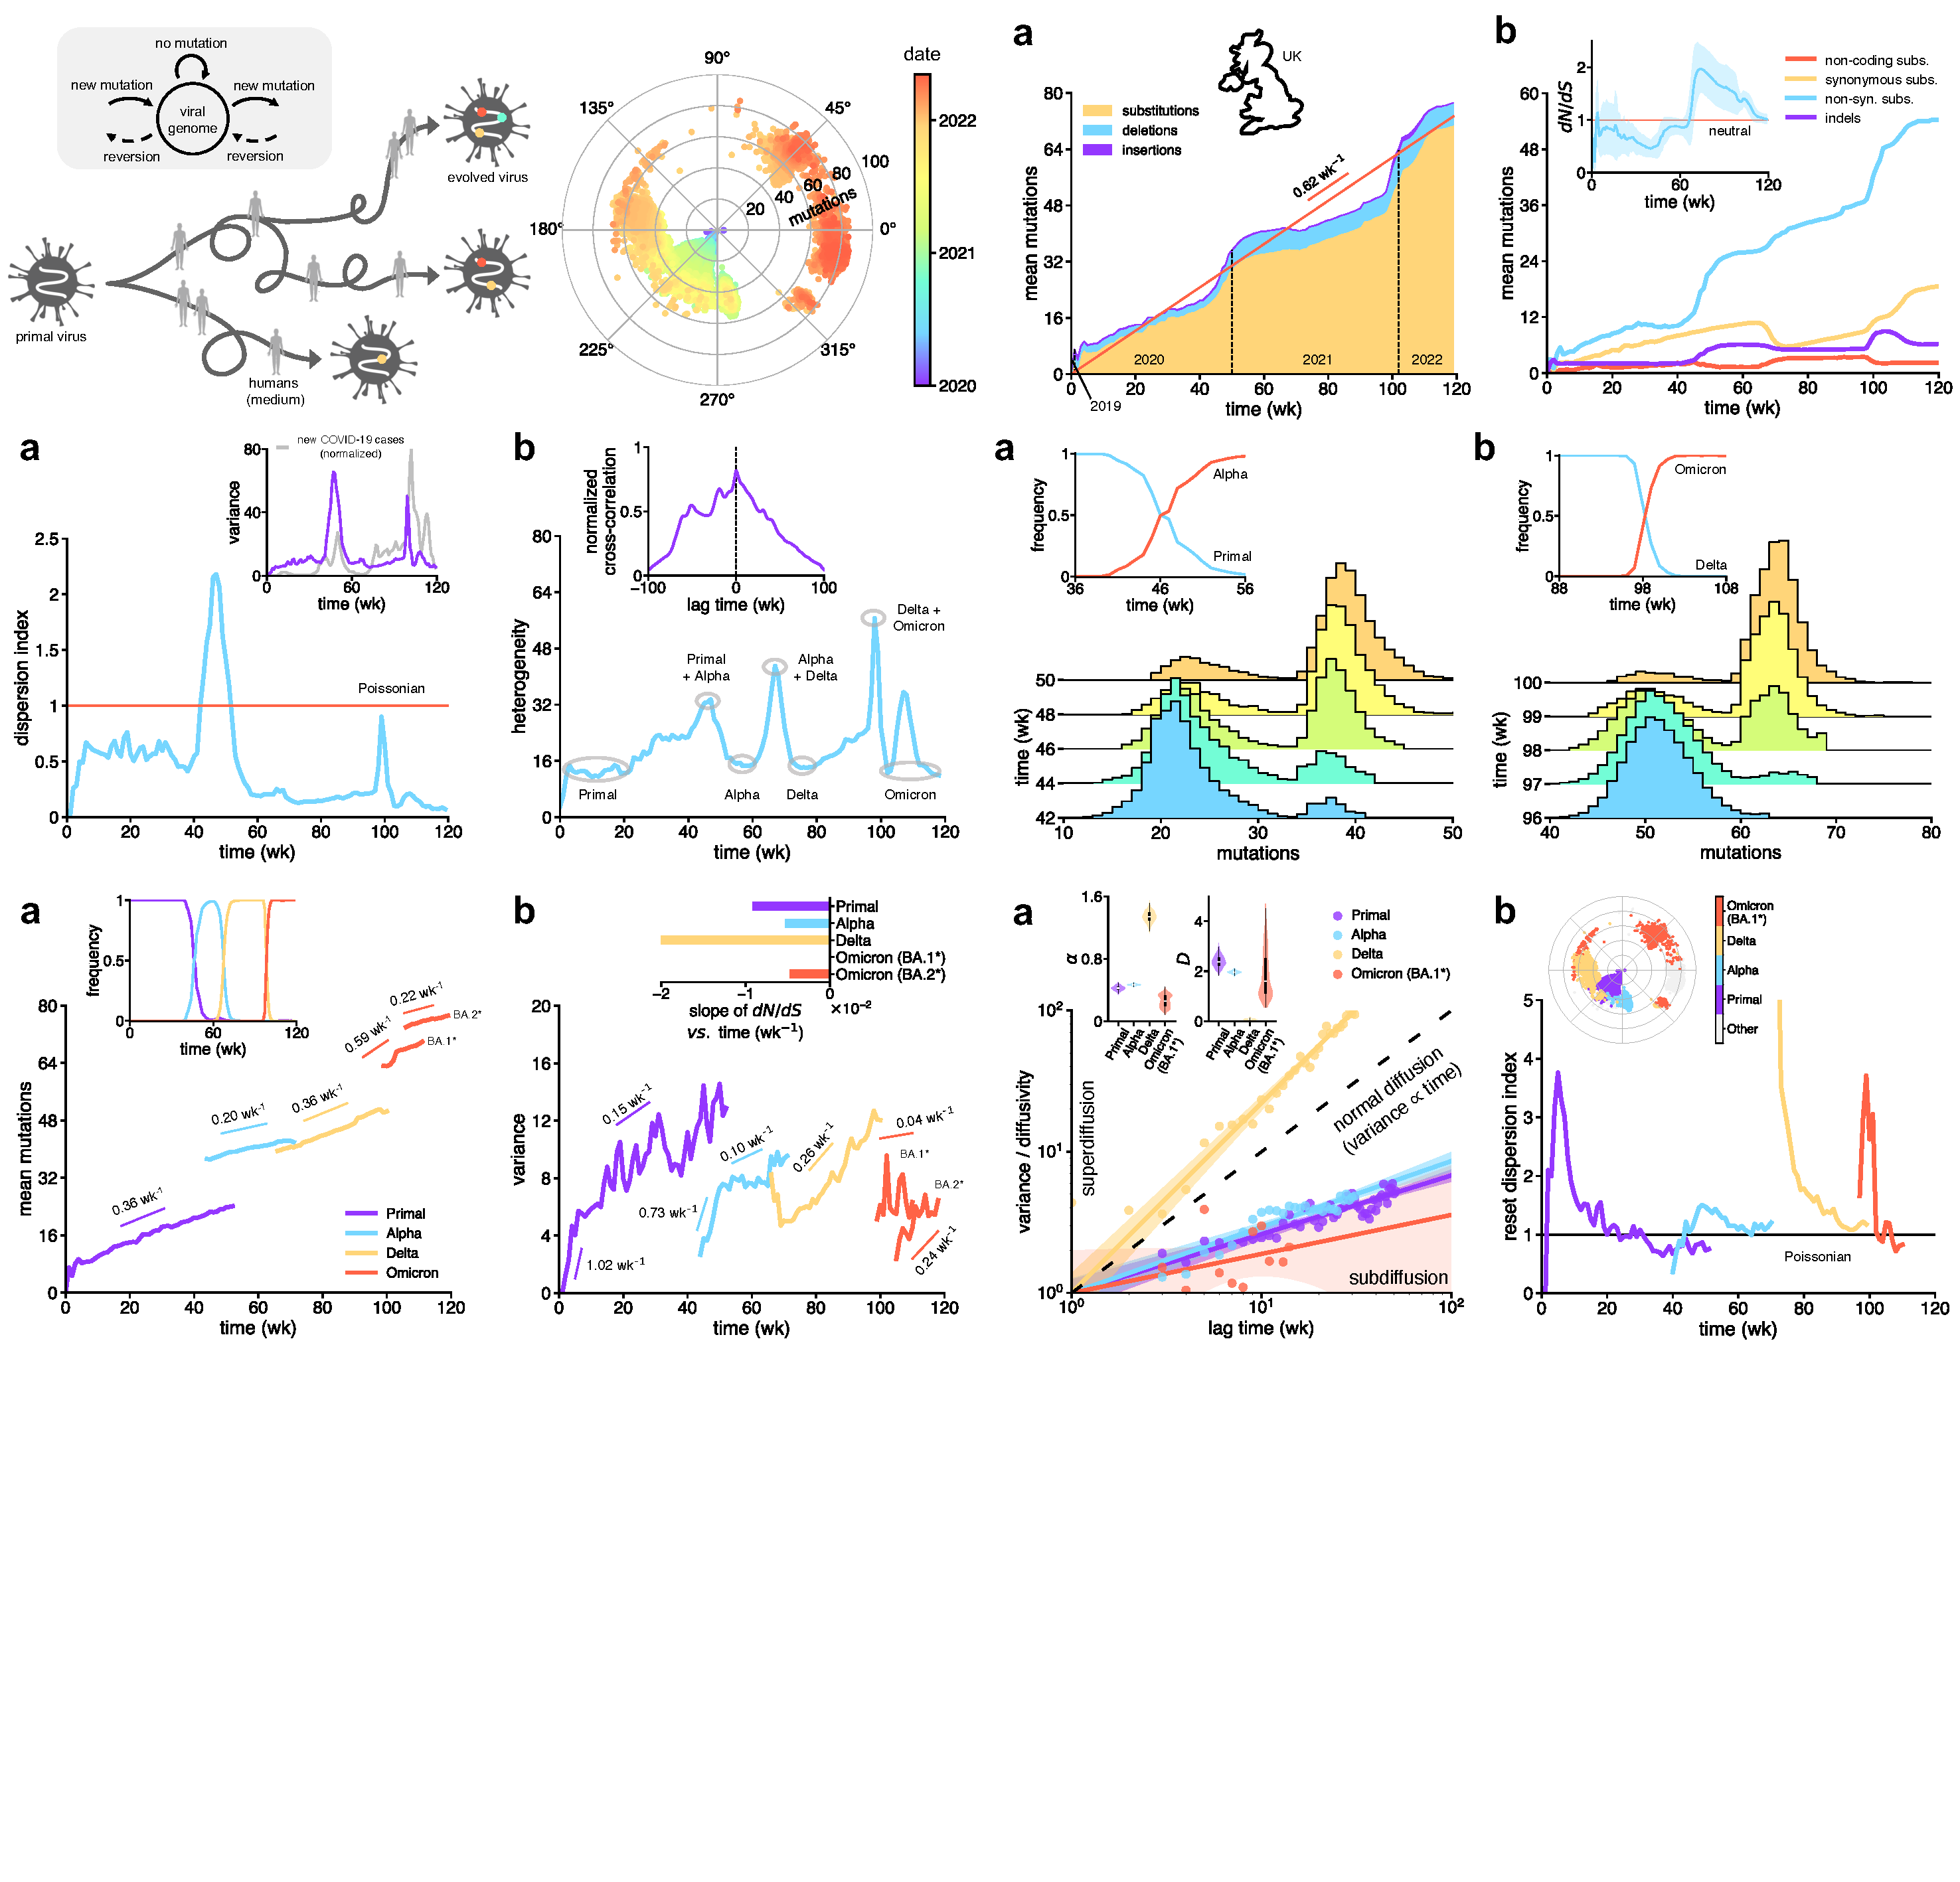
\includegraphics[trim={0.2cm 13.5cm 25.35cm 22.5cm},clip, width=\linewidth]{assets/Ch2Fig.pdf}
    \caption{a) Time-course of the mean number of accumulated mutations per variant (Omicron decomposed into BA.1 and BA.2). Linear regressions shown in each case (R\textsuperscript{2} $\geq$ 0.90). Inset: population frequency of the variants with time. b) Time-course of the variance per variant. Piecewise linear regressions shown in each case. Inset: slope of dN/dS with time for each variant obtained by linear regression.}\label{fig:fig2.6}
\end{figure}

To inspect the origin of anomalous diffusion in evolutionary motion, the rate at which the dN/dS ratio changed with time was analyzed per variant (inset of \textbf{Fig. \ref{fig:fig2.6}b}). We observed a decreasing trend in all cases, more pronounced for Delta. This suggested that Delta evolved by accumulating more synonymous mutations per site than the other variants. If these mutations were neutral \cite{deMaio2021}, the evolved genotypes of Primal, Alpha, and Omicron BA.1 would be more constrained as a result of their non-synonymous mutations, thereby explaining, at least in part, the observed subdiffusion patterns. Furthermore, we calculated a reset dispersion index, considering the accumulation of mutations since the appearance of the variant of study (\textit{i.e.}, each time a new variant invades the population, the number of mutations is reset). At long times, we found values in the neighborhood of 1, revealing an asymptotic Poissonian behavior following this metric (\textbf{Fig. \ref{fig:fig2.7}b}).

\begin{figure}[t]
    \centering
    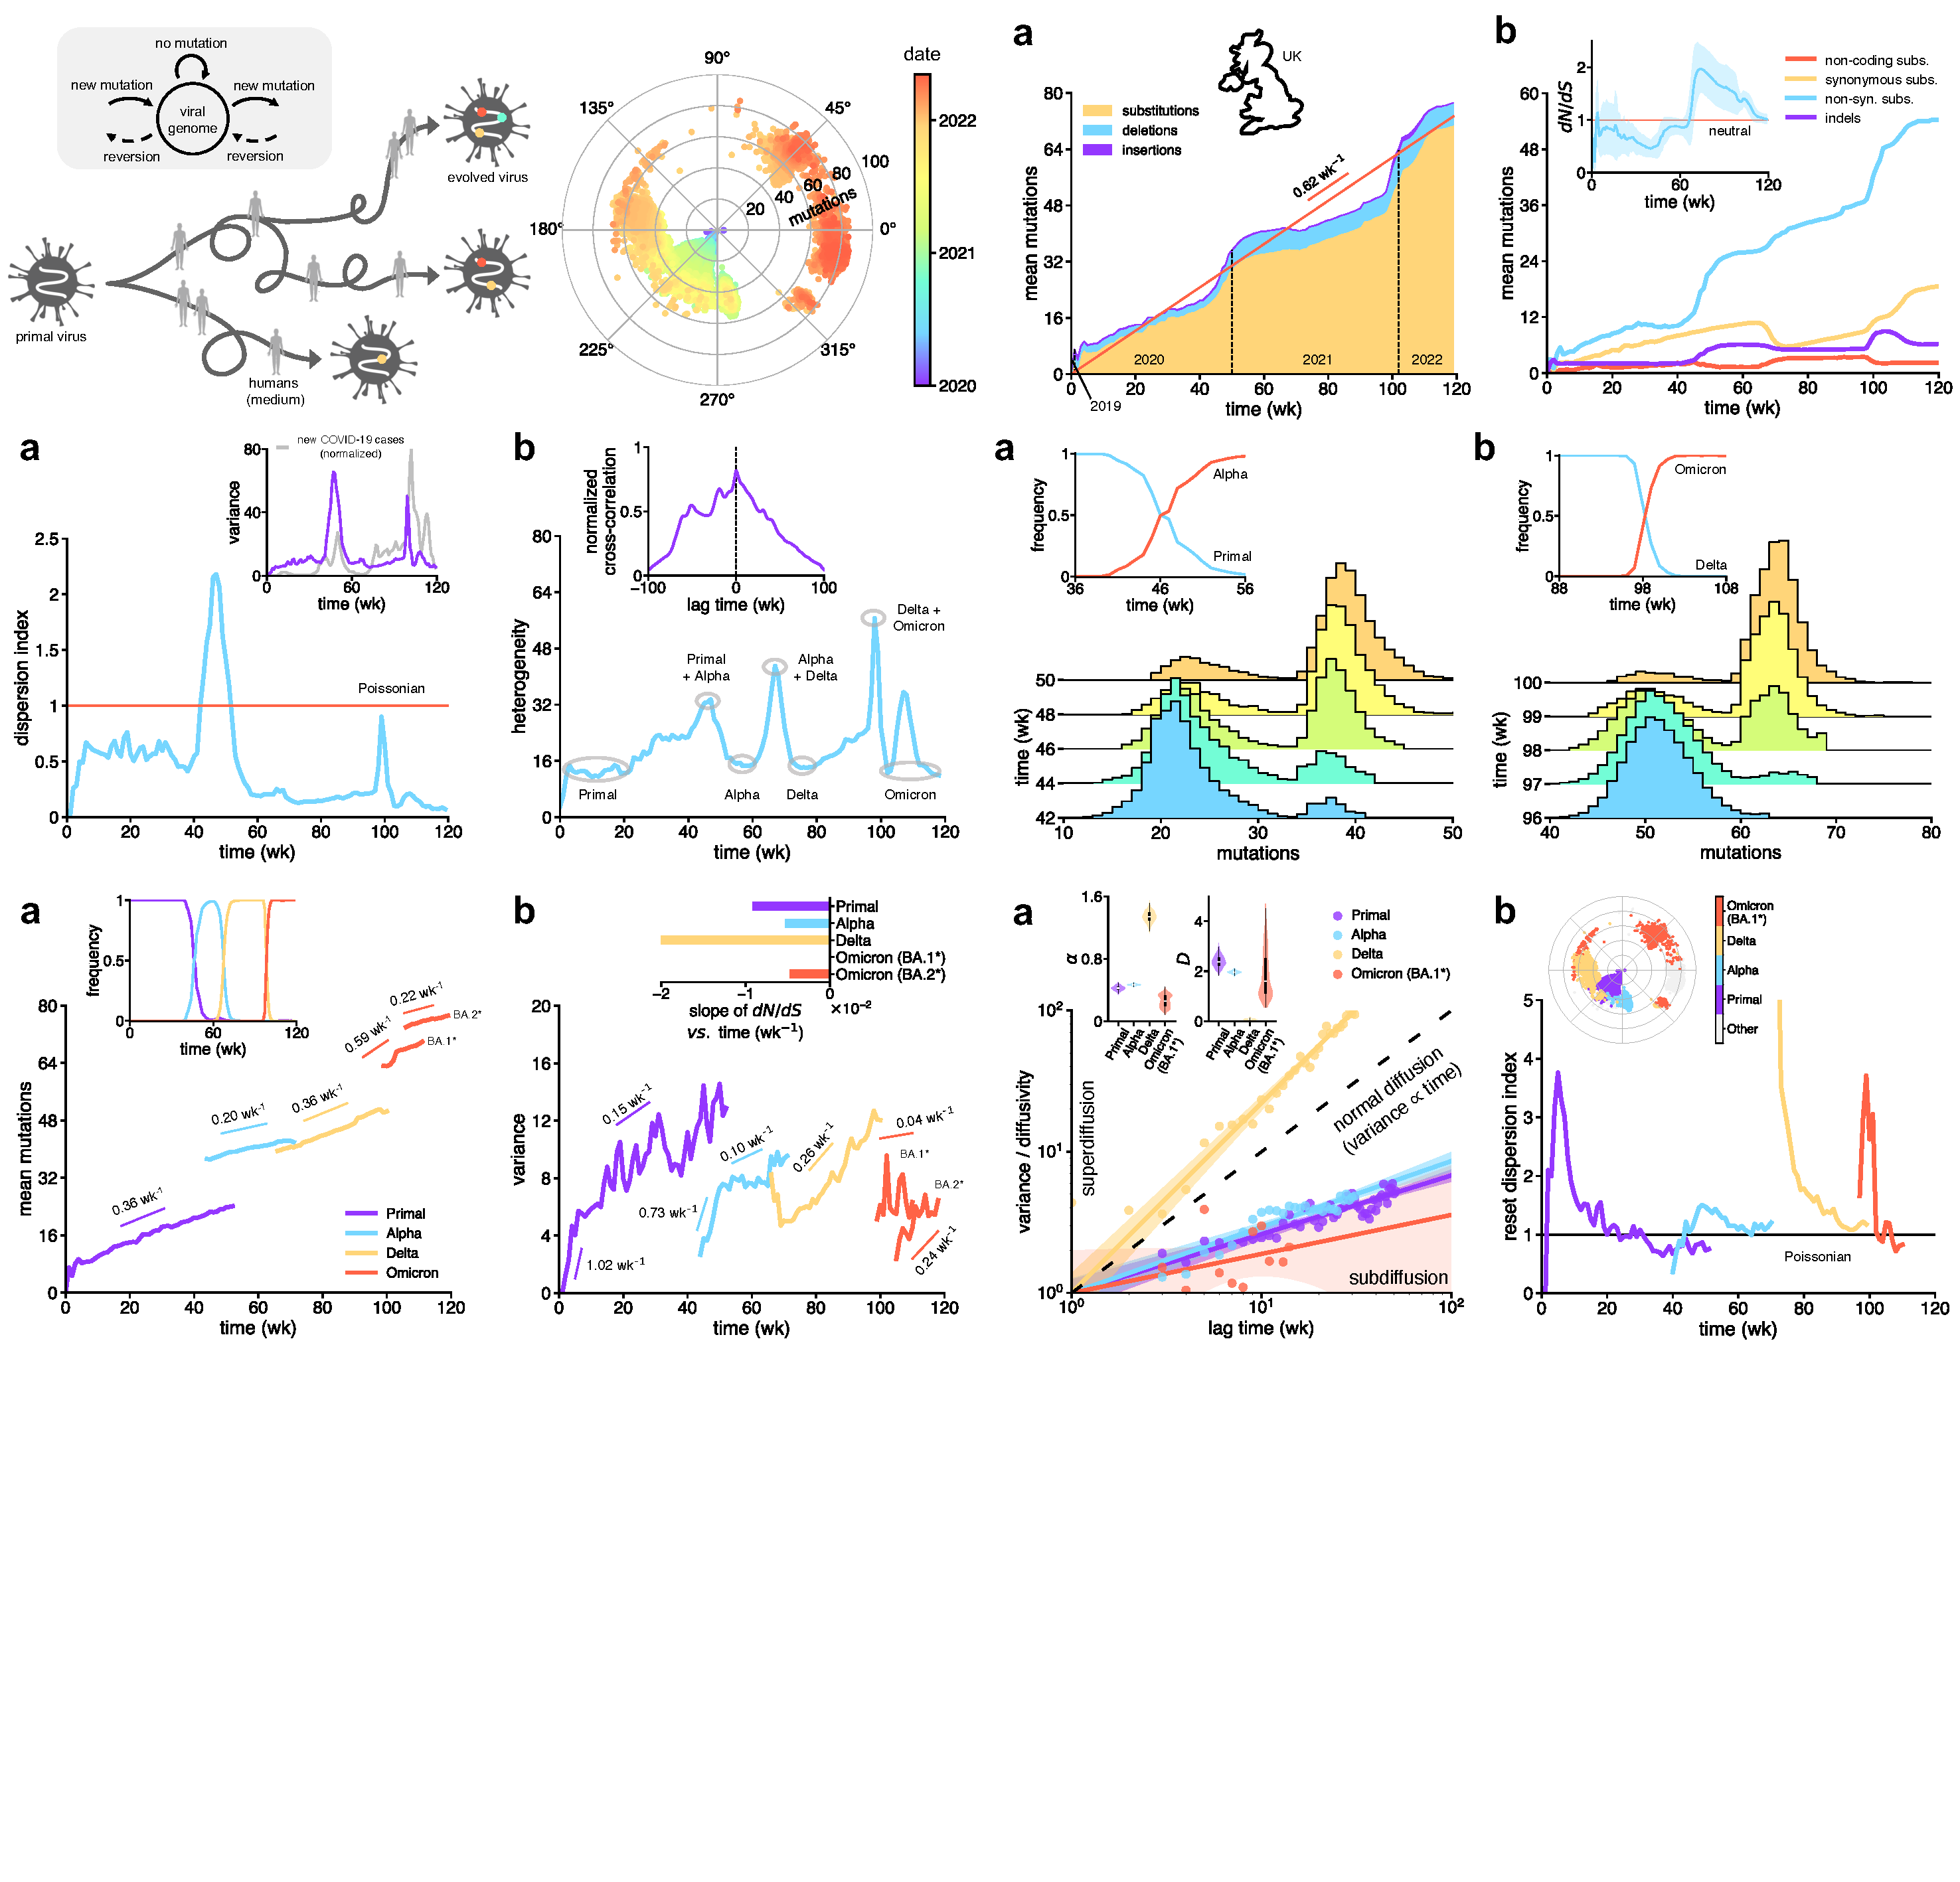
\includegraphics[trim={25.8cm 13.5cm 0.1cm 22.7cm},clip, width=\linewidth]{assets/Ch2Fig.pdf}
    \caption{a) Representation of the rescaled variance normalized by the diffusivity ($D$) with time in log scale (points correspond to data; for Primal, Alpha, Delta, and Omicron BA.1, R\textsuperscript{2} = 0.87, 0.88, 0.94, and 0.37, respectively, relative to Pearson's correlations in log scale). The slope of the fitted lines ($\alpha$) defines the type of diffusion ($\alpha>1$ superdiffusion, $\alpha<1$ subdiffusion). Shaded areas represent the 95\% confidence intervals of the regression lines. Inset: distributions of values for each diffusion parameter (violin plots) obtained by bootstrapping. b) Time-course of the reset dispersion index per variant. Inset: 2D projection of all viral sequences colored by variant (projection as in \textbf{Fig. \ref{fig:fig2.2}}). The variant-specific analyses were restricted to the time period in which their population frequency was at least 10\%.}\label{fig:fig2.7}
\end{figure}

\section{Discussion}

The observation of patterns of anomalous diffusion in biology has opened new avenues of research \cite{manzo2015}. Intriguingly, recent studies in which the physical movement of single SARS-CoV-2 virions was monitored throughout the infectious cycle highlighted transient and variant-dependent directionality and confinement outside and inside the cell \cite{christie2022, kreutzberger2022}, indicating deviation from a pure Brownian motion. Here, we have presented a new application domain in evolution. Of note, we uncovered that a probabilistic model with constant variant-dependent evolution rate and nonlinear mutational variance with time explained the SARS-CoV-2 evolutionary motion in humans during the first 120 weeks of pandemic in UK. This model might be used to refine phylodynamic approaches aimed at understanding the spread and adaptation of the virus. As shown, canonical descriptions based on the Poisson distribution do not accurately capture the observed dispersion at all time points.

These findings can also be situated within classical evolutionary theory, particularly Fisher's geometric model (FGM), which provides a quantitative framework to describe how organisms adapt in high-dimensional trait spaces.

\begin{definition}[Fisher's Geometric Model]
    Fisher's Geometric Model (FGM) conceptualizes the phenotype of an organism as a point $x \in \mathbb{R}^n$ in an $n$-dimensional Euclidean trait space, where each dimension represents an independent quantitative trait under stabilizing selection. The phenotypic optimum, corresponding to maximal fitness, is located at the origin of this space. The fitness of a phenotype $x$ is given by:
    
    \begin{equation}
        W(x) = W_0 \exp\left(-\frac{\|x\|^2}{2\sigma^2}\right),
    \end{equation}
    
    where $W_0 > 0$ denotes the maximal attainable fitness, $\sigma^2$ controls the strength of stabilizing selection (i.e., the curvature of the fitness landscape), and $\|x\|^2$ is the squared Euclidean distance from the phenotypic optimum. Mutational effects are modeled as random, isotropic displacements in phenotype space. The model predicts that the probability of a mutation being beneficial decreases as the phenotype approaches the optimum and increases with trait-space dimensionality $n$.
\end{definition}
    

Mutations correspond to random displacements $\Delta x$ in phenotype space, drawn from a symmetric distribution. The likelihood that a mutation increases fitness decreases with proximity to the optimum and increases with dimensionality $n$, due to the geometry of high-dimensional spaces. As a result, FGM predicts a declining rate of adaptation as populations approach a fitness peak \cite{couce2015}, along with a predominance of small-effect beneficial mutations. These properties make it a useful null model for interpreting adaptive dynamics in evolving populations \cite{tenaillon2014}.

In light of FGM, our findings offer both congruences and challenges. The subdiffusive mutational dynamics observed for Alpha and Omicron BA.1 variants are consistent with populations exploring a constrained phenotypic region near a fitness optimum, where evolutionary motion becomes increasingly restricted, an outcome that aligns with FGM's expectation of diminishing returns on adaptation. In contrast, the weak superdiffusive behavior seen in Delta reflects a more expansive phenotypic trajectory, possibly indicating that this variant originated from a population still far from the optimum and with greater adaptive potential. However, the punctuated emergence of variants with large mutational jumps, often involving dozens of substitutions, suggests evolutionary leaps not easily reconciled with FGM's assumption of small-effect mutations and a static fitness landscape \cite{miller2011}. These deviations may stem from shifts in host immunity, transmission dynamics, or selective pressures that effectively relocate the optimum over time. Furthermore, FGM's assumption of isotropic, additive mutational effects is likely violated in the context of SARS-CoV-2, where epistasis and context-dependent interactions are pervasive.

While FGM provides a valuable conceptual scaffold for interpreting our results within classical evolutionary theory, it falls short of fully capturing the complexity of SARS-CoV-2 dynamics. A more complete model would require generalizations that account for moving or rugged fitness landscapes, pervasive epistasis, and non-additive mutational effects, factors increasingly recognized as central to viral evolution. In parallel it is worth to note the bias in this type of studies caused by the fact that most of the sequenced viral genomes came from symptomatic infected people. Another issue is the imbalance in sequencing effort among countries, which prevents performing comprehensive analyses at a global scale. Further studies are required to assess the potential impact of movement and contact restrictions, vaccination, and self-diagnostic testing on the observed dynamic patterns. Overall, we anticipate deep implications of our data-driven results for future evolutionary and genomic studies, especially when dealing with fast evolving biological agents such as viruses.


\section{Materials and Methods}

\subsection{Whole-genome sequencing data}

The nucleotide sequences of the SARS-CoV-2 genomes used in this study were retrieved from the GISAID database (\url{https://www.gisaid.org}). As of May 2022, 10791877 sequences and the corresponding metadata were downloaded. Our analysis was restricted to the data from UK, which consists of 2735543 sequences. 

\subsection{Pairwise sequence alignments}

The nucleotide sequences of the SARS-CoV-2 genomes were aligned against a reference genome by means of Multiple Alignment using Fast Fourier Transform (MAFFT) \cite{katoh2002}. The results were collected in Clustal format. In this work, the reference sequence (root) was \texttt{hCoV-19/Wuhan/IVDC-HB-01/2019} (\texttt{EPI\_ISL\_402119}), which has 100\% identity with the GeneBank reference genome (\texttt{NC\_045512.2}) as shown by a Clustal Omega \cite{sievers2011} alignment.

\subsection{Construction of a functional dataset}

For each sequence, the number of mutations (substitutions, insertions, and deletions) with respect to the reference SARS-CoV-2 genome were counted. This information was retrieved from the MAFFT output alignments. In addition, the sequence collection dates and Pangolin lineages were retrieved from the metadata. Next, the sequences with unreliable recorded dates, whose unresolved base content surpassed 1\% (proportion of \texttt{N}s), or whose size was below 25 kb were discarded, as they were considered of low quality. Duplicated entries in the dataset were also removed. Furthermore, sequences isolated from non-human hosts were discarded. Then, the variant names were assigned where applicable based on the Pangolin lineage annotation. The Pangolin lineage-to-variant mapping was performed with information available at the Cov-lineages initiative (\url{https://cov-lineages.org}). All sequences dated earlier than 21 February 2021 were annotated as Primal variant (\textit{i.e.}, the original SARS-CoV-2 variant from Wuhan). The sequences were grouped by weeks. Finally, for each week, mutation outliers were filtered out to avoid artifacts in the calculated statistical parameters. These outliers could originate from incorrect date annotations, aberrant evolutionary trajectories, or sudden point introduction \cite{hill2022, michaelsen2022}. For each week, if the number of sequences was greater than 20, a Generalized Extreme Studentized Deviate (GESD) many-outlier procedure was applied \cite{rosner1983}. Otherwise, a filtering based on interquartile ranges was performed (\textit{i.e.}, the upper/lower bound was equal to the first/third quartile point plus/minus the interquartile range).

All data analyses were performed in Python using the libraries Pandas (\url{https://pandas.pydata.org}), NumPy (\url{https://numpy.org}), SciPy (\url{https://scipy.org}), Scikit-learn (\url{https://scikit-learn.org}), and Biopython (\url{https://biopython.org}).

\subsection{Landmark multidimensional scaling} %%% Ampliar?

Landmark multidimensional scaling (LMDS) is a variation of classical multidimensional scaling (MDS) \cite{mead1992} used to analyze and visualize dissimilarities between items based on a set of pairwise distance measures. The technique uses a small number of landmark items to compute their pairwise distances and estimate the distances between the remaining items, which are then mapped into a low-dimensional space using MDS \cite{deSilva2003}. LMDS presents several advantages over traditional MDS, including reduced computational complexity, scalability, and flexibility, making it an appropriate tool for analyzing large and complex datasets.

LMDS and principal component analysis (PCA) are both techniques used for dimensionality reduction, but they have some fundamental differences in their goals and methods. In contrast to LMDS, PCA is used to identify the underlying structure in a dataset by finding the principal components that explain the most variance in the data, capturing this way the most important patterns in the data \cite{jolliffe2016}. The interpretation of the coordinates in the projection space of both techniques is different as well, with PCA representing the patterns of variation and MDS representing the similarities and dissimilarities among the data points.

To obtain a representation of all available sequences in a two-dimensional (2D) space, a procedure based on landmark multidimensional scaling (LMDS) was followed \cite{deSilva2003}. For that, the Hamming distance between any two sequences was calculated (given by the number of mutations that separate each other). Metric axioms (minimality, symmetry, and triangle inequality) hold for the Hamming distance, so LMDS can be applied. The following sequences were used as landmarks:

\begin{table}[ht!]
    \centering
    \begin{tabular}{|l|l|}
        \hline
        \small\texttt{hCoV-19/England/CAMC-C42AEA/2020} & \small\texttt{hCoV-19/England/LSPA-2E824E8/2021}\\
        \small\texttt{hCoV-19/England/PHEC-YYBI3UW/2021} & \small\texttt{hCoV-19/Scotland/NORT-YBF4CD/2021}\\
        \small\texttt{hCoV-19/England/LSPA-3DC3179/2022} & \small\texttt{hCoV-19/England/ALDP-3A3CE1D/2022}\\
        \small\texttt{hCoV-19/England/ALDP-2E0DCFC/2021} & \small\texttt{hCoV-19/Wales/PHWC-PYDUBM/2021}\\
        \small\texttt{hCoV-19/England/QEUH-F8AA01/2021} & \small\texttt{hCoV-19/Scotland/QEUH-9AD0C0/2020}\\
        \hline
    \end{tabular}
    \caption{Sequence identifiers of landmarks employed during LMDS analysis.}
\end{table}

Polar coordinates were used to project the sequences in a 2D space. For the sake of interpretability, the radius was directly the total number of mutations from root and the angle was obtained from the coordinates generated by LMDS. It is worth noting that the position of two sequences in the projection plane will be determined by their similarity according to the Hamming distance. Consequently, if two sequences have the same number of mutations but these mutations are different, they will be located in different regions of the plane (i.e., their angles will be different and the radius will be the same).


\subsection{Calculation of statistical parameters}

For each set of SARS-CoV-2 sequences in a week, the mean and variance of the number of accumulated mutations (including substitutions and indels) were computed. For this computation, only the number of mutations was considered, not their type (\textit{i.e.}, different sequences with the same number of mutations counted the same). Then, the dispersion index was calculated, defined as the ratio between variance and mean. In addition, the mean Hamming distance between all sequence pairs in a week was computed to realize the extent of sequence heterogeneity. To compute the normalized cross-correlation between mutational variance and sequence heterogeneity, the \texttt{correlate} function from NumPy was used, having previously divided the statistical parameters by their norm (using the \texttt{linalg.norm} function). Finally, the number of COVID-19 cases in UK was retrieved from the database Our World in Data (\url{https://ourworldindata.org/}). The weekly number of new cases was computed. Probability-based histograms of the total number of mutations were obtained with the NumPy \texttt{histogram} function (\texttt{density=True}).

The calculation of mutational mean and variance was also performed per variant. This was done for the major lineages Primal, Alpha, Delta, and Omicron \cite{daCosta2022}, considering only the time period in which the variant represented at least the 10\% of the population. This limit was applied to avoid artifacts in the calculated statistical parameters due to a low number of sequences. In the case of Omicron, the calculation was performed for the sublineages BA.1 and BA.2 because of their great difference in mutations \cite{kumar2022}. For each variant, a reset dispersion index was also calculated, defined as the ratio between variance and the mean number of accumulated mutations since the first appearance of the variant in the population (\textit{i.e.}, each time a new variant invades the population, the number of mutations is reset). To some extent, this is in tune with the definition of a founder genotype for each clade from which to start counting as done in ref. \cite{neher2022}.

Specifically, if there are $N_k$ sequences in the $k$\textsuperscript{th} week, the mean number of accumulated mutations in that week, denoted by $\mathbb{E}\left[m_k\right]$, is calculated as follows:

\begin{equation}
    \mathbb{E}\left[m_k\right]=\frac{1}{N_k}\sum_{i=1}^{N_k}m_{k,i}\quad,
\end{equation}

\noindent where $m_{k,i}$ is the number of mutations of the $i$\textsuperscript{th} sequence in the $k$\textsuperscript{th} week. And the unbiased variance, denoted by $\mathbb{V}\left[m_k\right]$, is calculated as

\begin{equation}
    \mathbb{V}\left[m_k\right]=\frac{1}{N_k - 1}\sum_{i=1}^{N_k}\left(m_{k,i}-\mathbb{E}\left[m_k\right]\right)^2.
\end{equation}

To perform the calculations for a particular variant $v$, only the sequences annotated as such were considered (note that one sequence is linked at most to one particular variant). If there are $N_{v,k}$ sequences in the $k$\textsuperscript{th} week for variant $v$, the mean number of accumulated mutations in that week, denoted by $\mathbb{E}\left[m_{v,k}\right]$ is calculated as

\begin{equation}
    \mathbb{E}\left[m_{v,k}\right]=\frac{1}{N_{v,k}}\sum_{i=1}^{N_{v,k}}m_{v,k,i}\quad,
\end{equation}

\noindent where $m_{v,k,i}$ is the number of mutations of the $i$\textsuperscript{th} sequence in the $k$\textsuperscript{th} week annotated as variant $v$. And the variance, denoted by $\mathbb{V}\left[m_{v,k}\right]$, is calculated as

\begin{equation}
    \mathbb{V}\left[m_{v,k}\right] = \frac{1}{N_{v_k}-1}\sum_{i=1}^{N_{v,k}}\left(m_{v,k,i}-\mathbb{E}\left[m_{v,k}\right]\right)^2.
\end{equation}

Given that each sequence either belongs to a single variant, or to none, as a corollary of the above definitions the following relation holds:

\begin{equation}
    N_k=\sum_{v\in V}N_{v,k}+N_{\emptyset,k},
\end{equation}

\noindent where $V$ is the set of variants and $N_{\emptyset,k}$ denotes the number of sequences that are not linked to any variant of $V$ in the $k$\textsuperscript{th} week.

To assess the dispersion dynamics of the mutation distribution, the dispersion index ($\rho$) is used.

\begin{definition}[Dispersion Index]\label{def:dispersion_index}
    Given a stochastic process \( X(t) \) with finite mean \( \mathbb{E}\left[X(t)\right] \) and variance \( \mathbb{V}\left[X(t)\right] \), the Dispersion Index \( \rho(t) \), also known as the Fano Factor, is a measure of the relative variability of the process and is defined as

    $$
    \rho(t) = \frac{\mathbb{V}\left[X(t)\right]}{\mathbb{E}\left[X(t)\right]}
    $$
\end{definition}

\noindent Following \textbf{Definition \ref{def:dispersion_index}}, the dispersion index in the $k$\textsuperscript{th} week ($\rho_k$) is calculated as

\begin{equation}
    \rho_k=\frac{\mathbb{V}\left[m_{v,k}\right]}{\mathbb{E}\left[m_{v,k}\right]},
\end{equation}

\noindent and the reset dispersion index in the $k$\textsuperscript{th} week ($\rho_k^\text{reset}$) as

\begin{equation}
    \rho_k=\frac{\mathbb{V}\left[m_{v,k}\right]}{\mathbb{E}\left[m_{v,k}\right] - \mu_v},
\end{equation}

\noindent where $\mu_v$ is the mean number of mutations in the week in which $\mathbb{V}\left[m_{v,k}\right]$ is minimal. This condition corresponded to the first appearance of the variant of study in the population for Primal (first instance 26 Jan 2020), Alpha (first instance 25 Oct 2020), and Omicron BA.1 (first instance 21 Nov 2021), according to our functional dataset. In the case of Delta, however, the date of minimal variance did not coincide with the date of first instance, but rather with the moment at which the AY.4 lineage became dominant (16 May 2021) after a first period of time of selection within the Delta population, so this date was used for the mutation count reset.

\subsection{Global \textit{vs}. variant-based analysis}

The global analysis was carried out considering all available sequences from our functional dataset (\textit{i.e.}, pooling together the sequences even if they corresponded to different variants to compute the mean and variance for each week). This analysis served to appreciate the overall evolutionary trajectory by which the observable viral genome accumulates mutations with time in UK. That is, it allowed having a bird's eye perspective. More in detail, we could calculate a macroscopic evolution rate by linear regression between mean and time, and we could evaluate the dispersion dynamics of the resulting mutation distribution by representing the variance/mean ratio with time.

By contrast, the variant-based analysis was carried out considering only the sequences corresponding to a given variant, according to the annotation. This was done for Primal, Alpha, Delta, and Omicron (distinguishing also between the BA.1 and BA.2 lineages). Our analysis showed alternation of periods of evolution at lower rates and bursts of dispersion due to invasion events. We acknowledge that previous work already showed changes in the evolution rate with time in the particular case of SARS-CoV-2 \cite{ghafari2022, tay2022}. However, because our study was not based on phylogeny, we were able to process all available sequences in the database, gaining accuracy. In addition, and most importantly, because the dynamic profile of the variance was also analyzed, we were able to disclose anomalous diffusion patterns. This is a notable result that may contribute to change our understanding of virus evolution.

\subsection{Comparison with phylogenetic methods}

While in this work we are interested in how a viral population evolves, phylogenetic approaches mainly focus on genotypic differences in order to reconstruct evolutionary paths. Phylogenetic methods have been applied to produce estimates of the SARS-CoV-2 evolution rate, reporting values of 0.3-0.4 wk\textsuperscript{-1} during the first year of pandemic \cite{ghafari2022, wang2022}. These values are in tune with our calculations in the case of Primal. This congruence suggested us the formation with time of a sufficiently heterogenous viral population. Indeed, using the metric of heterogeneity, once a variant was fixed, the divergence between two arbitrary sequences of the population was about 11-15 mutations.

Further phylogenetic inferences have pointed out a transient increase of the evolution rate concomitant with the emergence of new invading variants (e.g., Alpha) \cite{tay2022}. However, by restricting the study to the sequences within the clade, the evolution rate did not appear to increase but rather to be maintained or even reduced (e.g., in the cases of Alpha and Delta). According to our analysis and also others in the field following non-phylogenetic approaches \cite{neher2022}, Alpha evolved a bit slower than Primal and Delta did at a similar rate. Despite the uncertainty associated with the emergence of new variants \cite{hill2022}, viral population- based studies are useful to understand the mutation-selection dynamics.

\subsection{Categorization of mutations}

For each viral sequence present in the functional dataset, the set of substitutions with respect to root were broken down into several categories: non-coding substitutions (\textit{i.e.}, substitutions that fall on non-coding regions of the genome), synonymous substitutions (\textit{i.e.}, substitutions that fall on coding regions but do not trigger amino acid changes), and non-synonymous substitutions (\textit{i.e.}, substitutions that trigger amino acid changes in coding regions). Insertions and deletions were counted into a unique variable called indels. Finally, the weekly mean and variance in terms of number of non-coding substitutions, synonymous substitutions, non-synonymous substitutions, and indels were computed.

\subsection{Estimation of natural selection signatures}

The ratio between the number of nonsynonymous and synonimous substitutions per site (dN/dS) was used to realize the sense of natural selection \cite{nielsen2005} during SARS-CoV-2 evolution, as it is a suitable statistical parameter to estimate the balance between positive (adaptive), neutral, and negative (purifying) selection acting on a set of protein-coding genes \cite{kryazhimskiy2008}. A simple method was employed to estimate the dN/dS ratio for each viral sequence \cite{nei1986}, assuming that:

\begin{enumerate}[i]
    \item The total length of the protein-coding genes was constant (equal to that of the reference genome).
    \item The four nucleotides had equal frequencies.
    \item The substitution events were random.
\end{enumerate}

First, the total number of synonymous ($S$) and non-synonymous ($N$) sites was estimated. Given that the probability of maintaining the same amino acid sequence is 5\% if the substitution occurs at the first position of the codon, 0\% if it occurs at the second position, and 72\% if it occurs at the third position, it turns out that $S\approx (0.05+0.72)R$  and $N\approx 3(R-S)$, where $R$ is the total length in base pairs of the protein-coding genes. Then, the proportion of synonymous ($p_S$) and non-synonymous ($p_N$) substitutions per site were computed. Second, these proportions were corrected to account for multiple potential changes at the same site. The genetic distance of synonymous ($d_S$) and non-synonymous ($d_N$) substitutions per site was estimated using the Jukes-Cantor formula. 

\begin{definition}[Jukes-Cantor Formula]
    Assuming equal base frequencies and equal probability of substition occurrence between any pair of nucleotides, the genetic distance can be approximated by

    $$
    d = -\frac{3}{4} \ln{\left(1 - \frac{4}{3}p\right)}
    $$

    where \(d\) is the estimated number of substitutions per site, and \(p\) is the observed proportion of nucleotide sites at which the two sequences differ \cite{jukes1969}.

    For the particular cases of synonymous (\(d_S\)) and non-synonymous (\(d_N\)) substitutions, the expression becomes

    $$
    \begin{cases}
        d_S = -\frac{3}{4} \ln{\left(1 - \frac{4}{3}p_S\right)}\\
        d_N = -\frac{3}{4} \ln{\left(1 - \frac{4}{3}p_N\right)}
    \end{cases}
    $$

    where \(p_S\) and \(p_N\) are the observed proportions of synonymous and non-synonymous nucleotide differences, respectively.
\end{definition}



\subsection{Mathematical modeling of evolutionary motion}

To motivate the development of a novel molecular clock model, we will briefly explore how a Poisson point process can be employed to model DNA sequence evolution. We then extend the Poisson point process into a continuous stochastic process, and finally present a model that captures the anomalous diffusion patterns observed in the evolutionary motion of SARS-CoV-2.

\subsubsection{Evolution as a Poisson point process}

The Poisson distribution is commonly used to model the occurrence of infrequent events within a fixed time or space interval. In the context of genetic mutations during DNA replication, each generation (defined as a replicative cycle) can introduce changes or substitutions in the DNA sequence due to various factors like errors induced by the DNA polymerase, radiation, or the presence of chemicals. Since the likelihood of a mutation at a specific position in the DNA sequence is assumed to be small, constant, and independent between generations (as supported by experimental evidence), the number of mutations in a lineage over $n$ generations can be accurately described using the Poisson distribution.



Let $u$ be the rate of mutations per generation, and $n$ the number of generations. In this scenario, the number of mutations that occur in a lineage during these $n$ generations follows a Poisson distribution with a mean value of $un$. In addition, if each generation takes the same amount of time, the number of mutations in the lineage during a specific time period $t$ can be described as a homogeneous Poisson point process, denoted as $\left\{N(t), t \geq 0\right\}$, where $N(t)$ represents the total number of mutations that have taken place up to (and including) time $t$. Consequently, the probability of observing exactly $n$ mutations, denoted as $N(t) = n$ at time $t$, is given by

\begin{equation}
    \text{Pr}(N(t) = n) = \frac{e^{-\kappa t}\left(\kappa t\right)^n}{n!}\label{eq:poisson},
\end{equation}

\noindent where $\kappa$ the rate of substitutions for a given unit of time. Importantly, \textbf{Equation \ref{eq:poisson}} implies that the number of mutations in a lineage at time $t = 0$ is $0$ and that the increments of the process are independent.

For further developments, it is convenient to compute the moment generating function, $M_{N(t)}(s)$, of the Poisson process:

\begin{align}
    M_{N(t)}(s) &= \mathbb{E}\left[e^{sN(t)}\right]\\
    &= \sum_{n=0}^{\infty} e^{sn} \frac{e^{-\kappa t}\left(\kappa t\right)^n}{n!}\nonumber\\
    &= e^{-\kappa t} \sum_{n=0}^{\infty} \frac{\left(\kappa t e^s\right)^n}{n!}\nonumber\\
    &= e^{-\kappa t} e^{\kappa t e^s}\nonumber\\
    &= e^{\kappa t (e^s - 1)}\label{eq:mgf}
\end{align}

By means of \textbf{Equation \ref{eq:mgf}} it is straightforward to demonstrate that the mean and variance of the process are both given by $\kappa t$:

\begin{align}
    \mathbb{E}\left[N(t)\right] &= \left.\frac{\partial}{\partial s}M_{N(t)}(s)\right|_{s=0}\\
    &= \left[\kappa t e^{\kappa t\left(e^s-1\right) + s}\right]_{s=0}\nonumber\\
    &= \kappa t\\
    \mathbb{V}\left[N(t)\right] &= \mathbb{E}\left[\left(N(t) - \mathbb{E}\left[N(t)\right]\right)^2\right]\\
    &= \mathbb{E}\left[N^2(t) -2N(t)\mathbb{E}\left[N(t)\right] + \mathbb{E}\left[N(t)\right]^2\right]\nonumber\\
    &= \mathbb{E}\left[N^2(t)\right] -\mathbb{E}\left[N(t)\right]^2\nonumber\\
    &= \left.\frac{\partial^2}{\partial s^2}M_{N(t)}(s)\right|_{s=0} - \left(\kappa t\right)^2\nonumber\\
    &= \left[\kappa t \left(\kappa t e^s + 1\right)e^{\kappa t\left(e^s - 1\right) + s}\right]_{s=0} - \left(\kappa t\right)^2\nonumber\\
    &= \left(\kappa t\right)^2 + \kappa t - \left(\kappa t\right)^2\nonumber\\
    &= \kappa t
\end{align}

As a corollary, and recalling \textbf{Definition \ref{def:dispersion_index}}, it is possible to assess that the process' dispersion index $\rho_{N(t)}$ is equal to $1$.

\subsubsection{Evolution approximated as a continuous stochastic process}\label{sec:evolution-approximated-as-a-continuous-stochastic-process}

Similar to how the Poisson distribution can be approximated by a Gaussian distribution through the central limit theorem, a Poisson point process can be approximated by a Wiener process. The Wiener process, also known as Brownian motion, is a continuous-time stochastic process characterized by independent and stationary increments. It is usually represented as $\left\{W(t), t \geq 0\right\}$, where $W(t)$ is a random variable representing the displacement of a particle at time $t$, its increments follow a normal distribution with a mean $\mathbb{E}[W(t)] = 0$ and, if it's the standard Wiener process, a covariance function $\text{Cov}[W(t), W(s)] = \min\left(t,s\right)$. The Wiener process is widely used as a model for random fluctuations in various physical systems.

Therefore, the number of mutations during DNA replication can be thought of a kind of \textit{random motion}, which we call \textit{evolutionary motion}, in the abstract space of all possible DNA sequences and it is defined as the following Langevin stochastic differential equation

\begin{equation}
    \frac{dm(t)}{dt} = \kappa + \sqrt{\kappa}\zeta(t)\label{eq:langevin},
\end{equation}

\noindent where $\zeta(t)$ is a Gaussian white noise characterized by $\mathbb{E}\left[\zeta(t)\right]=0$ and covariance function $\text{Cov}\left[\zeta(t),\zeta(s)\right]=\delta (t - s)$. Note that $\zeta(t)$ is defined as the formal derivative of the standard Wiener process $W(t)$, an assertion which has to be handled with caution because the Wiener process is nowhere differentiable with probability 1, therefore the Langevin formalism needs to be interpreted in a distributional sense. \textbf{Equation \ref{eq:langevin}} can be solved analytically:

\begin{align}
    \frac{dm(t)}{dt} &= \kappa + \sqrt{\kappa}\zeta(t)\nonumber\\
    m(t) &= m(0) + \kappa t + \sqrt{\kappa}\int_0^t \zeta(s)ds\label{eq:langevin-solution-dna}
\end{align}

\textbf{Equation \ref{eq:langevin-solution-dna}} can be further simplified given the number of mutations at time $t = 0$ is $0$:

\begin{align}
    m(t) &= m(0) + \kappa t + \sqrt{\kappa}\int_0^t \zeta(s)ds\nonumber\\
    &= \kappa t + \sqrt{\kappa}\int_0^t \zeta(s)ds\label{eq:langevin-solution-dna-simplified}
\end{align}

Note that the reformulation given at \textbf{Equation \ref{eq:langevin}}, which results in the solution at \textbf{Equation \ref{eq:langevin-solution-dna-simplified}}, maintains the original Poisson process' mean and variance:

\begin{align}
    \mathbb{E}\left[m(t)\right] &= \mathbb{E}\left[\kappa t + \sqrt{\kappa}\int_0^t \zeta(s)ds\right]\\
    &= \kappa t + \sqrt{\kappa}\mathbb{E}\left[\int_0^t\zeta(s)ds\right]\label{eq:langevin-mean-step1}\\
    &= \kappa t + \sqrt{\kappa}\int_0^t\mathbb{E}\left[\zeta(s)\right]ds\label{eq:langevin-mean-step2}\\
    &= \kappa t\label{eq:langevin-mean}
\end{align}

\begin{align}
    \mathbb{V}\left[m(t)\right] &= \mathbb{E}\left[\left(m(t) - \mathbb{E}\left[m(t)\right]\right)^2\right]\\
    &= \mathbb{E}\left[\left(\kappa t + \sqrt{\kappa}\int_0^t \zeta(s)ds - \kappa t \right)^2\right]\nonumber\\
    &= \kappa\mathbb{E}\left[\left(\int_0^t \zeta(s)ds\right)\left(\int_0^t \zeta(u)du\right)\right]\label{eq:langevin-variance-substep-a}\\
    &= \kappa\mathbb{E}\left[\int_0^t\int_0^t \zeta(s)\zeta(u)dsdu\right]\label{eq:langevin-variance-substep-b}\\
    &= \kappa\int_0^t\int_0^t \mathbb{E}\left[\zeta(s)\zeta(u)\right]dsdu\label{eq:langevin-variance-substep-c}\\
    &= \kappa\int_0^t\int_0^t \text{Cov}\left[\zeta(s),\zeta(u)\right]dsdu\label{eq:langevin-variance-substep-d}\\
    &= \kappa\int_0^t\int_0^t \delta(s-u) dsdu\label{eq:langevin-variance-substep-e}\\
    &= \kappa\int_0^t1du\nonumber\\
    &= \kappa t\label{eq:langevin-variance}
\end{align}

Note that the steps that involve \textbf{Equations \ref{eq:langevin-mean-step1}, \ref{eq:langevin-mean-step2}, \ref{eq:langevin-variance-substep-a}, \ref{eq:langevin-variance-substep-b}} and \textbf{\ref{eq:langevin-variance-substep-c}} are consequence of Fubini's theorem, which allows the interchange of the order of integration, as the integrals are known to be absolutely convergent and the fact that the expectation is a linear operator. The step that involves \textbf{Equations \ref{eq:langevin-variance-substep-c}} and \textbf{\ref{eq:langevin-variance-substep-d}} are consequence of the definition of covariance. The step that involves \textbf{Equations \ref{eq:langevin-variance-substep-d}} and \textbf{\ref{eq:langevin-variance-substep-e}} is a consequence of the definition of the Dirac delta functional. \textit{While the same result can be obtained through Itô's formalism, we will continue using Langevin's formalism due to its particular relevance in Biology.}

As a corollary, the corresponding dispersion index $\rho_{m(t)}$ remains equal to $1$ as expected, since the Wiener process is a continuous-time approximation of the Poisson process. One concern that arises from this reformulation is that the number of mutations $m(t)$ is no longer an integer, hence the model may not seem suitable for counting mutations in a lineage during a specific time period $t$. However, this issue can be easily solved by applying a rounding function to $m(t)$ whenever it is necessary to obtain an integer value.

\subsubsection{Anomalous Diffusion}

In the preceding section we demonstrated that, according to the molecular clock hypothesis, the number of mutations occurring in a lineage during a specific time period $t$ can be described as a Brownian motion (\textbf{Equation \ref{eq:langevin-solution-dna-simplified}}) exhibiting a mean and variance equal to $\kappa t$ (\textbf{Equations \ref{eq:langevin-mean}} and \textbf{\ref{eq:langevin-variance}}), where $\kappa$ represents the rate of substitutions for a given unit of time, akin to a microscopic particle moving in a fluid as a consequence of thermal forces.

However, it is well known that the diffusion of microscopic particles in a fluid does not always conform to Brownian motion. In fact, the diffusion of particles in a fluid can be classified into three main categories depending on their mean squared displacement (MSD; also understood as the variance of the stochastic process governing the motion): normal diffusion, subdiffusion, and superdiffusion. Under normal diffusion, the MSD of the particle is proportional to $t$, while under subdiffusion and superdiffusion the MSD of the particle is proportional to $t^\alpha$, where $\alpha$ is known as the diffusion exponent, with $\alpha < 1$ for the former case and $\alpha > 1$ for the latter \cite{munoz2021}.

Similarly to a microscopic particle moving in a fluid, the number of mutations in a lineage during a specific time period $t$ may not conform to a Brownian motion, as described by several studies observing overdispersed and underdispersed populations. Therefore, it is reasonable to consider that the number of mutations in a lineage during a specific time period $t$ may exhibit anomalous diffusion.

\subsubsection{Evolution as a fractional Brownian motion}

Multiple stochastic definitions of anomalous diffusion exist, and it is usually left to the researcher to use the one that best fits their problem. In this work, fractional Brownian motion (fBm) is used as a model for anomalous diffusion due to its simple yet powerful mathematical properties.

\begin{definition}[Fractional Brownian Motion]
    A fractional Brownian motion (fBm; denoted as $W_\alpha(t)$) is a continuous-time stochastic process that generalizes classical Brownian motion (Wiener process). It is characterized by stationary increments, mean $\mathbb{E}\left[W_\alpha(t)\right]=0$, and a covariance function of the form $\text{Cov}\left[W_\alpha(t),W_\alpha(s)\right] = \frac{1}{2}\left(t^\alpha + s^\alpha - |t-s|^\alpha\right)$, where $\alpha\in\left(0,2\right)$ is the diffusion exponent which determines the degree of long-term dependence of the process. It is related to the Hurst exponent $H$ by $\alpha = 2H$.
\end{definition}

It is straightforward to see that the Wiener process is a special case of the fBm, as the covariance function of the Wiener process is recovered when $\alpha = 1$. To reformulate the number of mutations in a lineage during a specific time period $t$ as a fBm, we will modify the Langevin stochastic differential equation shown in \textbf{Equation \ref{eq:langevin}}:

\begin{equation}
    \frac{dm(t)}{dt} = \kappa + \sqrt{\kappa}\eta(t)\label{eq:langevin-fbm},
\end{equation}

\noindent where $\eta(t)$ is an appropriate noise source characterized by $\mathbb{E}\left[\eta(t)\right]=0$ and a covariance function such that $\text{Cov}\left[W_\alpha(t),W_\alpha(s)\right] = \int_0^t\int_0^s\text{Cov}\left[\eta(u),\eta(v)\right]dudv$. Therefore, we interpret $\eta (t)$ as the generalized derivative of the fBm $W_\alpha(t)$, specifically we define

$$
\eta(t) := \frac{dW_\alpha(t)}{dt}
$$

\noindent in the distributional sense. Since $W_\alpha(t)$ is not differentiable in the classical sense when $\alpha\neq 1$, the above operation is understood via the action of tempered distributions on test functions in $\mathcal{S}(\mathbb{R})$ (the Schwartz space).

\begin{definition}[Schwartz space]
    The Schwartz space $\mathcal{S}(\mathbb{R})$ is the space of all infinitely differentiable functions $f:\mathbb{R}\to\mathbb{R}$ such that for all $k,l\in\mathbb{N}$ the function $x^k\frac{d^l}{dx^l}f(x)$ is rapidly decreasing, i.e., $\sup_{x\in\mathbb{R}}\left|x^k\frac{d^l}{dx^l}f(x)\right| < \infty$.
\end{definition}

\noindent By differentiating the covariance function of $W_\alpha(t)$ twice, with respect to $t$ and $s$, we obtain the covariance function of $\eta(t)$. It is straightforward to see that $\frac{\partial^2}{\partial t\partial s}\text{Cov}\left[W_\alpha(t),W_\alpha(s)\right]$ is equivalent to computing $-\frac{1}{2}\frac{\partial^2}{\partial t\partial s}|t-s|^\alpha$ given that the terms $t^\alpha$ and $s^\alpha$ end up vanishing during the differentiation. To ease subsequent computations, we define the following change of variables:

$$
\begin{cases}
    x &= t - s\\
    \partial_t &= \partial_x\\
    \partial_s &= -\partial_x
\end{cases}
$$

therefore

\begin{align*}
    -\frac{1}{2}\frac{\partial^2}{\partial t\partial s}|t-s|^\alpha &= -\frac{1}{2}\frac{\partial^2}{\partial t\partial s}|x|^\alpha\\
    &= \frac{1}{2}\frac{d^2}{dx^2}|x|^\alpha
\end{align*}

\noindent again, understood in the distributional sense. Let $g(x) = |x|^\alpha$ and $\psi(x)\in\mathcal{S}(\mathbb{R})$ be a test function, the second distributional derivative of $g(x)$ is defined as

\begin{equation}
    \left\langle g'',\psi\right\rangle = \int_{-\infty}^{\infty}g''(x)\psi(x)dx\label{eq:distributional_derivative_definition}
\end{equation}

Using integration by parts and the property that $\psi(x)$ is rapidly decreasing, we obtain

\begin{align}
    \left\langle g'',\psi\right\rangle &= \int_{-\infty}^{\infty}g''(x)\psi(x)dx\nonumber\\
    &= \left[g'(x)\psi(x)\right]_{-\infty}^{\infty} - \int_{-\infty}^{\infty}g'(x)\psi'(x)dx\nonumber\\
    &= 0 - \int_{-\infty}^{\infty}g'(x)\psi'(x)dx\nonumber\\
    &= -\left[g(x)\psi''(x)\right]_{-\infty}^{\infty} + \int_{-\infty}^{\infty}g(x)\psi''(x)dx\nonumber\\
    &= \int_{-\infty}^{\infty}g(x)\psi''(x)dx \label{eq:derivative_transferred}
\end{align}

By using the definition $g(x)$ and the integral's linearity, we can work back from \textbf{Equation \ref{eq:derivative_transferred}} an expression that parallels \textbf{Equation \ref{eq:distributional_derivative_definition}}:

\begin{align*}
    \int_{-\infty}^{\infty}g(x)\psi''(x)dx =& \int_{-\infty}^{\infty}\left|x\right|^\alpha \psi''(x)dx\\
    =& \int_{-\infty}^0(-x)^\alpha \psi''(x)dx + \int_{0}^{\infty}x^\alpha \psi''(x)dx\\
    =& \left[(-x)^\alpha\psi'(x)\right]_{-\infty}^0 + \int_{-\infty}^0\alpha(-x)^{\alpha - 1} \psi'(x)dx\\
    &+ \left[-x^\alpha\psi'(x)\right]_{0}^{\infty} - \int_{0}^{\infty}\alpha x^{\alpha - 1} \psi'(x)dx\\
    =& \int_{-\infty}^0\alpha(-x)^{\alpha - 1} \psi'(x)dx - \int_{0}^{\infty}\alpha x^{\alpha - 1} \psi'(x)dx\\
\end{align*}

\begin{align*}
    =& \left[\alpha(-x)^{\alpha-1}\psi(x)\right]_{-\infty}^0 + \int_{-\infty}^0\alpha(\alpha - 1)(-x)^{\alpha - 2} \psi(x)dx\\
    &+ \left[\alpha x^{\alpha - 1}\psi(x)\right]_{0}^{\infty} + \int_{0}^{\infty}\alpha(\alpha - 1)x^{\alpha - 2} \psi(x)dx\\
    =& \int_{-\infty}^0\alpha(\alpha - 1)(-x)^{\alpha - 2} \psi(x)dx + \int_{0}^{\infty}\alpha(\alpha - 1)x^{\alpha - 2} \psi(x)dx\\
    =& \int_{-\infty}^{\infty}\alpha(\alpha - 1)\left|x\right|^{\alpha - 2}\psi(x)dx\\
\end{align*}

Resulting in the following equivalence:

$$
\left\langle g'',\psi\right\rangle = \int_{-\infty}^{\infty}g''(x)\psi(x)dx = \int_{-\infty}^{\infty}\alpha(\alpha - 1)\left|x\right|^{\alpha - 2}\psi(x)dx
$$

So the distributional second derivative of $g(x)$ is equivalent to $\alpha(\alpha - 1)\left|x\right|^{\alpha - 2}$, which results in the following expression for the covariance function of $\eta(t)$:

\begin{equation}
\text{Cov}\left[\eta(t),\eta(s)\right] = \frac{1}{2}\alpha(\alpha - 1)\left|t-s\right|^{\alpha - 2}\label{eq:covariance-solved}
\end{equation}

This expression is a well defined generalized function (distribution) on $\mathbb{R}^2 \backslash \left\{t=s\right\}$, where the set of points $\left\{t=s\right\}$ represent a singularity. However, this singularity is integrable in the sense of distributions, so the integral $\text{Cov}\left[W_\alpha(t),W_\alpha(s)\right] = \int_0^t\int_0^s\text{Cov}\left[\eta(u),\eta(v)\right]dudv$ remains well defined. This definition allows for the computation of the appropriate mean and variance of the process (MSD of the evolutionary motion):

\begin{align}
    \mathbb{E}\left[m(t)\right] &= \mathbb{E}\left[\kappa t + \sqrt{\kappa}\int_0^t \eta(s)ds\right]\\
    &= \kappa t
\end{align}
\begin{align}
    \mathbb{V}\left[m(t)\right] &= \mathbb{E}\left[\left(m(t) - \mathbb{E}\left[m(t)\right]\right)^2\right]\\
    &= \kappa\mathbb{E}\left[\left(\int_0^t \eta(s)ds\right)^2\right]\nonumber\\
    &= \kappa\int_0^t\int_0^t\mathbb{E}\left[\eta(s)\eta(u)\right]dsdu\nonumber\\
\end{align}
\begin{align}
    &= \frac{\alpha\kappa}{2}(\alpha - 1)\int_0^t\int_0^t\left|s - u\right|^{\alpha - 2}dsdu\nonumber\\
    &= \frac{\alpha\kappa}{2}(\alpha - 1)\int_0^t\left[\int_0^u\left(u - s\right)^{\alpha - 2}ds + \int_u^t\left(s - u\right)^{\alpha - 2}ds\right]du\nonumber\\
    &= \frac{\alpha\kappa}{2}\int_0^t\left[s^{\alpha-1}+(t-s)^{\alpha - 1}\right]du\nonumber\\
    &= \kappa t^\alpha\label{eq:fbm-variance}
\end{align}

Therefore, by using fBm as a model for anomalous diffusion, the number of mutations in a lineage during a specific time period $t$ can be described as a stochastic process with a mean and variance equal to $\kappa t$ (in line with the molecular clock hypothesis \cite{ayala1999}) and $\kappa t^\alpha$, respectively. Therefore, the analysis of $\mathbb{V}\left[m(t)\right]$ with time is instrumental to assess the nature of the stochastic movement. Previous evolutionary studies of viruses mainly focused on the mean behavior \cite{jenkins2002,ghafari2022,neher2022,tay2022,wang2022}, i.e., evaluating the relationship $\mathbb{E}\left[m(t)\right]=\kappa t$, so our study is pertinent due to the completeness achieved.

Particularly, our model for the evolution of SARS-CoV-2 follows a more generalized approach, as it decouples the mean mutation rate from the diffusion coefficient (the latter also being $\kappa$ in \textbf{Equation \ref{eq:fbm-variance}}). Being $m(t)$ the number of accumulated mutations in the viral genome at time $t$, the stochastic differential equation introduced in \textbf{Section \ref{sec:results}}

\begin{equation}
    \frac{dm(t)}{dt}=\kappa + \xi (t)\tag{\ref{eq:solution-model}}
\end{equation}

\noindent governs the dynamics of the system. Here $\kappa$ is the evolution rate and $\xi (t)$ is an integrative noise source whose statistical properties match a fBm \cite{kursawe2013}:

\begin{equation}
    \begin{cases}
        \quad\mathbb{E}\left[\xi (t)\right] = 0\\
        \text{Cov}\left[\xi (t), \xi (s)\right] = \frac{1}{2}D\alpha\left(\alpha - 1\right)\left|t-s\right|^{\alpha - 2}
    \end{cases}.
\end{equation}

In this formulation, $D$ is the diffusion coefficient and $\alpha$ the diffusion exponent. Again, the solution for the mean evolutionary motion is

\begin{equation}
    \mathbb{E}\left[m(t)\right]=\kappa t,
\end{equation}

\noindent which is compatible to the molecular clock hypothesis \cite{ayala1999}. Linear regressions were performed between the calculated mean number of mutations in the viral sequences and time using the \texttt{LinearRegression} function from Scikit-learn. This was done for the global data and also for the major lineages Primal, Alpha, Delta, and Omicron (BA.1 and BA.2). Similar to the general model, the solution for the variance is

\begin{equation}
    \mathbb{V}\left[m(t)\right] = Dt^\alpha,
\end{equation}

\noindent which is compatible with the fBm model, as the MSD is then proportional to a power of time. However, this solution comes from a fixed initial condition (\textit{i.e.}, no variability at $t=0$). The calculated variance from the viral sequences was fitted to the general expression

\begin{equation}
    \mathbb{V}\left[m(t)\right] = \sigma_0^2 + Dt^\alpha,
\end{equation}

\noindent where $\sigma_0^2$ is a parameter that accounts for the initial variance in the population ($\sigma_0^2$ was directly computed from the set of sequences). Nonlinear regressions were performed between $\mathbb{V}\left[m(t)\right] - \sigma_0^2$ and time using the \texttt{curve\_fit} function from SciPy. This was done for the global data and also for the major lineages Primal, Alpha, Delta, and Omicron (BA.1). In the case of Delta, the variance analysis was restricted to the AY.4 sublineage, which was the dominant in UK after a first period of time in which other sublineages coexisted (the fixation of the AY.4 sublineage led to a decrease in variance).

% \subsection{Brownian \textit{vs}. non-Brownian motion}

% A Brownian motion is a continuous-space and continuous-time model to describe the stochastic movement of a free particle. Here, we considered a viral particle that moves in the space of sequences. If we denote by $\Delta m(t)$ the deviation from the mean behavior in terms of number of mutations, \textit{i.e.}, $\Delta m(t)=m(t)-\kappa t$, we can write

% \begin{equation*}
%     \frac{d\Delta m(t)}{dt}=\xi (t)
% \end{equation*}

% \noindent For $\Delta m(t)$ to be a Brownian motion, it must have a null mean displacement, \textit{i.e.}, $\left\langle\Delta m(t)\right\rangle = 0$, and a mean squared displacement (\textit{i.e.}, variance) proportional to time, \textit{i.e.}, $\left\langle\Delta m(t)^2\right\rangle\propto t$. A null mean displacement generally holds because typical noise sources obey $\left\langle\xi (t)\right\rangle=0$. In a scenario in which the mean squared displacement does not scale linearly with time, let us say $\left\langle\Delta m(t)^2\right\rangle\propto t^\alpha$ with $\alpha\neq 1$, the motion is said to be non-Brownian (the term anomalous diffusion is also used to refer to this scenario) \cite{manzo2015}.

% The properties of the noise source $\xi (t)$ determine the type of stochastic movement. In the typical case of Gaussian white noise, \textit{i.e.}, $\left\langle\xi (t)\right\rangle=0$ and $\left\langle\xi (t)\xi (t')\right\rangle=D\delta (t-t')$, where $\delta(t)$ is the Dirac delta function, it turns out that

% \vfill\pagebreak

% \begin{align*}
%     \left\langle\Delta m(t)^2\right\rangle &= \left\langle\int_0^t\int_0^t\xi(r)\xi(s)drds\right\rangle\\
%     &= \int_0^t\int_0^t\left\langle\xi(r)\xi(s)\right\rangle drds\\
%     &= D\int_0^t\int_0^t\delta(r-s)drds\\
%     &= Dt
% \end{align*}

% \noindent However, considering $\left\langle\xi(t)\xi(t')\right\rangle=\frac{1}{2}D\alpha(\alpha - 1)\left|t-t'\right|^{\alpha-2}$, it turns out that

% \begin{align*}
%     \left\langle\Delta m(t)^2\right\rangle &= \left\langle\int_0^t\int_0^t\xi(r)\xi(s)drds\right\rangle\\
%     &= \int_0^t\int_0^t \frac{1}{2}D\alpha(\alpha - 1)\left|r-s\right|^{\alpha-2} drds\\
%     &= \frac{1}{2}D\alpha(\alpha - 1)\int_0^t\left[\int_0^s (s-r)^{\alpha-2}dr+\int_s^t (r-s)^{\alpha-2}dr\right]ds\\
%     &= \frac{1}{2}D\alpha\int_0^t\left[s^{\alpha-1}+(t-s)^{\alpha-1}\right]ds\\
%     &= Dt^\alpha
% \end{align*}

\subsection{Statistical significance of the diffusion parameters}

Bootstrapping was applied to assess the robustness of the estimations of $D$ and $\alpha$. This approach resamples the original dataset with replacement to generate new bootstrap datasets. We can then fit the same model to each of these bootstrap datasets, obtaining a distribution of model parameters. This distribution can be used to estimate the variability of the model parameters and to evaluate the robustness of the model to small changes in the original dataset \cite{efron1979}. In this work, a random sampling with replacement of the sequences was performed each week. The sampling size was defined as the 50\% of the total number of sequences available in each week in the original dataset (\textit{i.e.}, if there are 100 sequences in a week, the bootstrap sample size for that week is 50, what is called subsampling). This was done for all 120 weeks in an independent manner. We chose a sample size that was large enough to capture the key characteristics of the original dataset, but small enough to make the bootstrap procedure computationally feasible and robust to observations with a disproportionate impact on the results. With the new bootstrap dataset, the mean and variance were calculated. This procedure was repeated 1000 times. As a result, a distribution of values for each diffusion parameter was obtained, having performed 1000 independent regressions. This was done for the major variants Primal, Alpha, Delta, and Omicron (BA.1).

\vfill

\pagebreak

\bibliographystyle{assets/rodrigostyle}
\bibliography{references/chapter2references}
